\documentclass[10pt]{memoir}
\setstocksize{220mm}{155mm} 	        
\settrimmedsize{220mm}{155mm}{*}	
\settypeblocksize{170mm}{116mm}{*}	
\setlrmargins{18mm}{*}{*}
\setulmargins{*}{*}{1.2}
%\setlength{\headheight}{5pt}%
\checkandfixthelayout[lines]
\linespread{1.16}
\flushbottom

%%% Hyphenation settings
\usepackage[htt]{hyphenat}
\hyphenation{he-lio-trope opos-sum}
\tracingparagraphs=1
%Hyphenation in Devanāgarī of the edition still missing? Probably this needs to be modified in babel-iast package? 

%%% babel
\usepackage[english]{babel}
\usepackage{babel-iast/babel-iast}

\babelfont[iast]{rm}[Renderer=Harfbuzz, Scale=1.3]{AdishilaSan}%AdishilaSan}
\babelfont[english]{rm}{Adobe Text Pro}

%%% more functionality
\PassOptionsToPackage{hyphens}{url}
\usepackage{hyperref}
\usepackage{pdflscape}
\usepackage{cleveref}
\usepackage{url}
\usepackage{cleveref}
\usepackage{microtype}
\usepackage{lineno}

%\usepackage{bigfoot}
%%% more functions
\usepackage[dvipsnames]{xcolor}
%\usepackage[para,perpage]{footmisc}

%%%für den Counter von Kapiteln und Sätzen! 
\newcommand{\uproman}[1]{\uppercase\expandafter{\romannumeral#1}}
\newcommand{\lowroman}[1]{\romannumeral#1\relax}

\makeindex
\newfontfamily\sanskritfont[Script=Devanagari,Mapping=RomDev,Scale=1.1]{Sanskrit2003}
\usepackage{pifont,fourier-orns,lettrine,psvectorian,paralist,enumitem,pdfpages,wrapfig,tabulary,lettrine,longtable}
\setlist[enumerate]{itemsep=0mm}
\usepackage[autostyle]{csquotes}
\usepackage[defaultlines=2,all]{nowidow}
\usepackage{ellipsis,adforn,booktabs,longtable,url,tikz}
\lineskiplimit=-3pt          

\makechapterstyle{IeT}{%
  \chapterstyle{default}
  \renewcommand*{\printchapternonum}{\centering}
  \renewcommand*{\clearforchapter}{\cleartorecto} 
  \aliaspagestyle{chapter}{empty}}
\chapterstyle{IeT}
\setsecnumdepth{none}  \openright  \nouppercaseheads
\settocdepth{subsubsection}

%%%% test better pagebreaks
%\def\fussy{%
%  \emergencystretch\z@
%  \tolerance 200%
%  \hfuzz .1\p@
%  \vfuzz\hfuzz}

%\interfootnotelinepenalty=10000\relax

%\usepackage[maxfloats=256]{morefloats}

%\maxdeadcycles=500

%raggedbottomsectiontrue
%%\checkandfixthelayout


%%%%%%%  biblatex
%\newcommand{\noun}[1]{\textsc{#1}}    %  philosophy-verbose
\usepackage[backend=biber, sorting=nyt, style=verbose]{biblatex} %%%%ORIGINAL TiE
\renewcommand*{\mkbibnamefamily}[1]{\textsc{#1}}


\DeclareFieldFormat{url}{%
  \mkbibacro{URL}\addcolon\space
  \href{#1}{\nolinkurl{\thefield{urlraw}}}}

\DeclareFieldFormat{citeurl}{%
  \href{#1}{\nolinkurl{\thefield{urlraw}}}} 


\DeclareFieldFormat{postnote}{#1}
\renewcommand{\postnotedelim}{, }
\addbibresource{bindu.bib}

%%% ekdosis
\usepackage[teiexport=tidy,parnotes=true]{ekdosis}% =tidy cleans up HTML and XML documents by fixing markup errors and upgrading legacy code to modern standards. parnotes=footnotes below or above critical apparatus

\SetLineation{lineation=page, modulo} %lineation=page sets thenumbering to start afresh at the top of each page. =modulo makes every fifth line numbered. {lineation=page} makes every line numbered! 

\renewcommand{\linenumberfont}{\selectlanguage{english}\footnotesize} %sets language of lines to English

\SetTEIxmlExport{autopar=false} %autopar=falseinstructs ekdosis to ignore blank lines in the.tex sourcefile as markers for paragraph boundaries. As a result, each paragraph of the edition must be found within an environment associated with the xml <p> element

\SetHooks{
  lemmastyle=\bfseries,
  %refnumstyle=\selectlanguage{english}\bfseries,
  refnumstyle=\selectlanguage{english}\color{blue}\bfseries,
  appheight=0.8\textheight,
}

\newif\ifinapparatus
\DeclareApparatus{source}[
%bhook=\inapparatustrue,
lang=english,
notelang=english,
% bhook=\selectlanguage{english},
bhook=\selectlanguage{english}\textbf{Sources:},%
%maxentries=4, 
%ehook=.]
%sep={] },
%nosep,
]

\newif\ifinapparatus
\DeclareApparatus{testium}[
%bhook=\inapparatustrue,
lang=english,
notelang=english,
% bhook=\selectlanguage{english},
bhook=\selectlanguage{english}\textbf{Testimonia:},
%maxentries=4, 
%ehook=.]
%nosep, 
]

% Declare \ifinapparatus and set \inapparatustrue at the beginning of
% the apparatus criticus block. Also set the language.  
\newif\ifinapparatus
  \DeclareApparatus{default}[
  %bhook=\inapparatustrue, 
  lang=english,
  %maxentries=33,
  %bhook=\selectlanguage{english},
  sep = {] },
  delim=\hskip 0.75em,
  rule=\rule{0.7in}{0.4pt},
]

\newif\ifinapparatus
\DeclareApparatus{philcomm}[
%bhook=\inapparatustrue,
lang=english,
notelang=english,
bhook=\selectlanguage{english}\textbf{Philological Commentary:},
%bhook=\selectlanguage{english},
sep={: },
]

\ekdsetup{
showpagebreaks,
spbmk = \textcolor{blue}{spb},
hpbmk = \textcolor{red}{hpb}
}

%\usepackage{fnpos}
%\makeFNmid
%\makeFNbottom
\usepackage[bottom]{footmisc}
%%%%%%%%%%%%%%%%%%%%%%%%%%%
\makeatletter
\def\blfootnote{\gdef\@thefnmark{}\@footnotetext}
\makeatother
%%%%%%%%%%%%%%%%%%%%%%%%%


% Macros and Definitions for the Print of Sigla
\def\acpc#1#2#3{{#1}\rlap{\textrm{\textsuperscript{#3}}}\textsubscript{\textrm{#2}}\space}
\def\sigl#1#2{{{#1}}\textsubscript{\textrm{#2}}}
\def\None{{\sigl{N}{1}}} \def\Noneac{\acpc{N}{1}{ac}\,} \def\Nonepc{\acpc{N}{1}{pc}\,}
\def\Ntwo{{\sigl{N}{2}}} \def\Noneac{\acpc{N}{2}{ac}\,} \def\Nonepc{\acpc{N}{2}{pc}\,}
\def\Done{{\sigl{D}{1}}} \def\Doneac{\acpc{D}{1}{ac}\,} \def\Donepc{\acpc{D}{1}{pc}\,}
\def\Dtwo{{\sigl{D}{2}}} \def\Dtwoac{\acpc{D}{2}{ac}\,} \def\Dtwopc{\acpc{D}{2}{pc}\,}
\def\Uone{{\sigl{U}{1}}} \def\Uoneac{\acpc{U}{1}{ac}\,} \def\Uonepc{\acpc{U}{1}{pc}\,}                 
\def\Utwo{{\sigl{U}{2}}} \def\Utwoac{\acpc{U}{2}{ac}\,} \def\Utwopc{\acpc{U}{2}{pc}\,}

%%%%%%%%%%%%%% Tattvabinduyoga - List of Witnesses   %%%%%%%%%%%%%%%%%%%
\DeclareWitness{ceteri}{\selectlanguage{english}cett.}{ceteri}[]   
\DeclareWitness{E}{\selectlanguage{english}E}{Printed Edition}[]    
\DeclareWitness{P}{\selectlanguage{english}P}{Pune BORI 664}[]  
\DeclareWitness{B}{\selectlanguage{english}B}{Bodleian 485}[]       
\DeclareWitness{N1}{\selectlanguage{english}N\textsubscript{1}}{NGMPP 38/31}[]
\DeclareWitness{N2}{\selectlanguage{english}N\textsubscript{2}}{NGMPP B 38/35}[]
\DeclareWitness{L}{\selectlanguage{english}L}{LALCHAND 5876}[]  
\DeclareWitness{D}{\selectlanguage{english}D}{IGNCA 30019}[] 
%\DeclareWitness{D2}{\selectlanguage{english}D\textsubscript{2}}{IGNCA 30020}[]  
\DeclareWitness{U1}{\selectlanguage{english}U\textsubscript{1}}{SORI 1574}[] 
\DeclareWitness{U2}{\selectlanguage{english}U\textsubscript{2}}{SORI 6082}[]
%%%%%%%%%%%%%% Tattvabinduyoga - Groups of Witnesses   %%%%%%%%%%%%%%%%%%%
\DeclareWitness{X}{\selectlanguage{english}\alpha}{Alpha Group: D,N1,N2,U1}[]
\DeclareWitness{Y}{\selectlanguage{english}\beta}{Beta Group: B,E,L,P,U2}[]
%%%%%%%%%%%%% Testimonia
\DeclareWitness{Ysv}{\selectlanguage{english}Ysv}{Yogasvarodaya}[] %%%add infos!  

%%%%%%%%%%%%%%%%%%%%%%%%%%%%%%%%%%%%%%%%%%%
% Macro for Editing Abbrevs.
\def\om{\textrm{\footnotesize \textit{om.}\ }} %prints om. for omitted in apparatus
\def\korr{\textrm{\footnotesize \textit{em.}\ }} %prints em. for emended in apparatus
\def\conj{\textrm{\footnotesize \textit{conj.}\ }} %prints conj. for conjectured in apparatus

% \supplied{text} EDITORIAL ADDITION -> Within \lem oder \rdg
% \surplus{text} EDITORIAL DELETION -> Within \lem oder \rdg
% \sic{text} CRUX
% \gap{text} LACUNAE -> [reason=??, unit=??, quantity=??, extent=??]


%%%%%%%%%%%%%%%%%%%%%%%%%%%%%%%%%%%%%%%%%%% All macros of this list can be used in 
% Macro for Editing Abbrevs.
\def\eyeskip{\textrm{{ab.\,oc. }}}
\def\aberratio{\textrm{{ab.\,oc. }}}
\def\ad{\textrm{{ad}}}
\def\add{\textrm{{add.\ }}}
\def\ann{\textrm{{ann.\ }}}
\def\ante{\textrm{{ante }}} 
\def\post{\textrm{{post }}}
%\def\ceteri{cett.\,}                   
\def\codd{\textrm{{codd.\ }}}

\def\coni{\textrm{{coni.\ }}}
\def\contin{\textrm{{contin.\ }}}
\def\corr{\textrm{{corr.\ }}}
\def\del{\textrm{{del.\ }}}
\def\dub{\textrm{{ dub.\ }}}

\def\expl{\textrm{{explic.\ }}} 
\def\explica t{\textrm{{explic.\ }}}
\def\fol{\textrm{{fol.\ }}}
\def\foll{\textrm{{foll.\ }}}
\def\gloss{\textrm{{glossa ad }}}
\def\ins{\textrm{{ins.\ }}}      
\def\inseruit{\textrm{{ins.\ }}} 
\def\im{{\kern-.7pt\lower-1ex\hbox{\textrm{\tiny{\emph{i.m.}}}\kern0pt}}} %\textrm{\scriptsize{i.m.\ }}}      
\def\inmargine{{\kern-.7pt\lower-.7ex\hbox{\textrm{\tiny{\emph{i.m.}}}\kern0pt}}}%\textrm{\scriptsize{i.m.\ }}}      
\def\intextu{{\kern-.7pt\lower-.95ex\hbox{\textrm{\tiny{\emph{i.t.}}}\kern0pt}}}%\textrm{\scriptsize{i.t.\ }}}           
\def\indist{\textrm{{indis.\ }}}  
\def\indis{\textrm{{indis.\ }}}
\def\iteravit{\textrm{{iter.\ }}} 
\def\iter{\textrm{{iter.\ }}}
\def\lectio{\textrm{{lect.\ }}}   
\def\lec{\textrm{{lect.\ }}}
\def\leginequit{\textrm{{l.n. }}} 
\def\legn{\textrm{{l.n. }}}
\def\illeg{\textrm{{l.n. }}}

\def\primman{\textrm{{pr.m.}}}
\def\prob{\textrm{{prob.}}}
\def\rep{\textrm{{repetitio }}}
\def\secundamanu{\textrm{\scriptsize{s.m.}}}            \def\secm{{\kern-.6pt\lower-.91ex\hbox{\textrm{\tiny{\emph{s.m.}}}\kern0pt}}}%   \textrm{\scriptsize{s.m.}}}
\def\sequentia{\textrm{{seq.\,inv.\ }}}  
\def\seqinv{\textrm{{seq.\,inv.\ }}}
\def\order{\textrm{{seq.\,inv.\ }}}
\def\supralineam{{\kern-.7pt\lower-.91ex\hbox{\textrm{\tiny{\emph{s.l.}}}\kern0pt}}} %\textrm{\scriptsize{s.l.}}}
\def\interlineam{{\kern-.7pt\lower-.91ex\hbox{\textrm{\tiny{\emph{s.l.}}}\kern0pt}}}   %\textrm{\scriptsize{s.l.}}}
\def\vl{\textrm{v.l.}}   \def\varlec{\textrm{v.l.}} \def\varialectio{\textrm{v.l.}}
\def\vide{\textrm{{cf.\ }}}
\def\cf{\textrm{{cf.\ }}} 
\def\videtur{\textrm{{vid.\,ut}}}
\def\crux{\textup{[\ldots]} }
\def\cruxx{\textup{[\ldots]}}
\def\unm{\textit{unm.}}
%%%%%%%%%%%%%%%%%%%%%%%%%%%%%%%%%%%%

% List of Scholars
\DeclareScholar{ego}{ego}[
forename=Nils Jacob,
surname=Liersch]

% Persons:14\DeclareScholar{ego}{ego}[15forename=Robert,16surname=Alessi]17% Useful shorthands:18\DeclareShorthand{codd}{codd.}{V,I,R,H}19\DeclareShorthand{edd}{edd.}{Lit,Erm,Sm}20\DeclareShorthand{egoscr}{\emph{scripsi}}{ego}

%Useful shorthands:
%\DeclareShorthand{codd}{codd.}{V,I,R,H}
%\DeclareShorthand{edd}{edd.}{Lit,Erm,Sm}
\DeclareShorthand{egoscr}{em.}{ego}
\DeclareShorthand{egoscrconj}{conj.}{ego}
\DeclareShorthand{egomute}{\unskip}{ego}

\usepackage{xparse}

\NewDocumentEnvironment{tlg}{O{}O{}}{\setlength{\leftskip}{0pt}\vspace{-1ex}\begin{quotation}}{\hfill #1\ \vspace{-1ex}\end{quotation}\vspace{-1ex}} %verse environment
%\NewDocumentEnvironment{tlg}{O{}O{}}{\begin{verse}}{॥#1\hskip-4pt ॥\\ \end{verse}}
\NewDocumentCommand{\tl}{m}{{\selectlanguage{iast} #1}}

\NewDocumentCommand{\extra}{m}{{\textcolor{gray}{#1}}} %command for additions to U2
\NewDocumentCommand{\crazy}{m}{{\textcolor{red}{#1}}} %totally corrupted passage
\NewDocumentCommand{\coro}{m}{{\textcolor{violet}{#1}}} %colour for sentence counter! 

\NewDocumentEnvironment{prose}{O{}}{\begin{otherlanguage}{iast}}{\end{otherlanguage}}
% \NewDocumentEnvironment{padd}{O{}}{\begin{otherlanguage}{iast}}{\end{otherlanguage}}
\NewDocumentEnvironment{tlate}{O{}}
%\NewDocumentEnvironment{tadd}{O{}}

%Define two commands: \skp ("sanskrit plus"), to be ignored by TeX in
%the edition text, but processed in the TEI output. Conversely, \skm
%("sanskrit minus") is to be processed in the edition text, but
%ignored if found in the apparatus criticus and in the TEI output:

\NewDocumentCommand{\skp}{m}{}
\TeXtoTEIPat{\skp {#1}}{#1}

%\NewDocumentCommand{\skpp}{m}{}
%\TeXtoTEIPat{\skpp {#1}}{#1}

\NewDocumentCommand{\skm}{m}{\unless\ifinapparatus#1-\fi}
\TeXtoTEIPat{\skm {#1}}{}

% \NewDocumentCommand{\dd}{}{/\hskip-4pt/}
\NewDocumentCommand{\dd}{}{\mbox{/\hskip-4pt/}}
\TeXtoTEIPat{\dd {}}{//}


%%% modify environments and commands
%%% TEI mapping
\TeXtoTEIPat{\begin {tlg}}{<lg>} %lg=(Group of verse (s)) contains one or more verses or lines of verse that together form a formal unit (e.g. stanza, chorus).
\TeXtoTEIPat{\end {tlg}}{</lg>}

\TeXtoTEIPat{\begin {prose}}{<p>}
\TeXtoTEIPat{\end {prose}}{</p>}

\TeXtoTEIPat{\begin {tlate}}{<p>}
\TeXtoTEIPat{\end {tlate}}{</p>}

\TeXtoTEIPat{\\}{}
\TeXtoTEIPat{\linebreak}{<br/>}
\TeXtoTEIPat{\noindent}{}
%\TeXtoTEI{tl}{l}
\TeXtoTEI{emph}{hi}
\TeXtoTEI{bigskip}{}
\TeXtoTEI{None}{N1}
\TeXtoTEI{Ntwo}{N2}
\TeXtoTEI{Done}{D1}
\TeXtoTEI{Dtwo}{D2}
\TeXtoTEI{Uone}{U1}
\TeXtoTEI{Utwo}{U2}
%\TeXtoTEIPat{/}{ |}
%\TeXtoTEI{//}{ ||}
\TeXtoTEIPat{\korr}{em. }
\TeXtoTEIPat{\conj}{conj.}
\TeXtoTEIPat{\om}{om.}
\TeXtoTEIPat{english}{}
\TeXtoTEIPat{\hskip}{}
\TeXtoTEIPat{\hskip-4pt}{}
\TeXtoTEIPat{\hskip-2pt}{}
\TeXtoTEIPat{-}{ }
\TeXtoTEIPat{4pt}{}
\TeXtoTEIPat{2pt}{}
\TeXtoTEIPat{\textcolor {#1}{#2}}{<hi rend="#1">#2</hi>} 

% Nullify \selectlanguage in TEI as it has been used in
% \DeclareWitness but should be ignored in TEI.
\TeXtoTEI{selectlanguage}{}



\FormatDiv{1}{\begin{center}\Large}{\end{center}}
\FormatDiv{2}{\begin{center}\small}{\end{center}}
\FormatDiv{3}{\bfseries}{.}
\title{Yogatattvabindu of Rāmacandra\\ A Critical Edition and Annotated Translation}
\date{\today}

\parindent=15pt
\begin{document}

% Zitiermöglichkeiten:
%\footcite[See][p.\,1]{goldstein01:_tibet_englis_diction_moder_tibet}
%\footnote{\cite{goldstein01:_tibet_englis_diction_moder_tibet}.}

\frontmatter
\thispagestyle{empty}
\begin{center}
  {\Large \emph{The Yogatattvabindu}}\\[3mm]
\end{center}



\newpage

\

\thispagestyle{empty}



\normalsize


\newpage


\begin{center}
\thispagestyle{empty}

\

\vskip 2mm

\begin{otherlanguage}{iast}
\LARGE \sanskritfont{Yogatattvabindu}
\end{otherlanguage}

\vskip .4cm

\Huge Yogatattvabindu \\[7mm]
\Large Critical Edition\\
with annotated Translation


\large

\vspace{3cm}

Von

Nils Jacob Liersch
\small
\vfill

\vfill

Indica et Tibetica Verlag \\ % $\cdot$ 
Marburg 2024

\vskip 6mm

\end{center}

\newpage
\newpage \ \thispagestyle{empty}
\small  \

\noindent

\
\vfill


\small
\noindent \textbf{Bibliographische Information Der Deutschen Bibliothek}

\noindent
Die Deutsche Bibliothek verzeichnet diese Publikation in der Deutschen Nationalbibliographie;
detaillierte bibliographische Informationen sind im Internet über http://dnb.ddb.de abrufbar.

\noindent
\textbf{Bibliographic information published by Die Deutschen Bibliothek}

\noindent
Die Deutsche Bibliothek lists this publication in the Deutsche Nationalbibliographie; detailed
bibliographic data is available in the Internet at http://dnb.ddb.de.  


\vskip 1cm

\noindent
\copyright\ Indica et Tibetica Verlag, Marburg 2024

\medskip

\noindent
Alle Rechte vorbehalten / All rights reserved

\medskip

\noindent
Ohne ausdrückliche Genehmigung des Verlages ist es nicht gestattet, das Werk oder einzelne Teile
daraus nachzudrucken, zu vervielfältigen oder auf Datenträger zu speichern.

\smallskip

\noindent
Apart from any fair dealing for the purpose of private study, research, criticism or review, no
part of this book may be reproduced or translated in any form, by print, photo form, microfilm, or
any other means without written permission. Enquiries should be made to the publishers.

\bigskip

\noindent
Satz: \ \ Nils Jacob Liersch \\
Herstellung: \ \ BoD – Books on Demand GmbH, Norderstedt  \\

\bigskip

\noindent
%\ISBN     

\normalsize

\newpage

%\maketitle
\clearpage
\tableofcontents
\addtocounter{page}{-1}
\thispagestyle{empty}
\clearpage


\mainmatter

\chapter{Conventions in the Critical Apparatus}
\section{Sigla in the Critical Apparatus}

\begin{itemize}
\item E : Printed Edition
\item P : Pune BORI 664
\item L : Lalchand Research Library LRL5876
\item B : Bodleian Oxford D 4587
\item \None : NGMPP B 38-31
\item \Ntwo : NGMPP B 38-35 / A 1327-14
\item \Done : IGNCA 30019
\item \Uone : SORI 1574
\item \Utwo: SORI 6082
\end{itemize}

\chapter{Critical Edition \& Annotated Translation}
\cleardoublepage
\begin{alignment}[
  texts=edition[class="edition"];
  translation[class="translation"],
  ]
  \begin{edition}
               \ekddiv{
   head={[\uproman{13}. \textbf{lakṣyayogaḥ}]},
 type=section,
 depth=2, 
 n=XIII
}
\xmlhead[h13]{[XIII. lakṣyayogaḥ]}
\label{laksyayoga}
    \begin{prose}[p13_01]
      \noindent
%------------------------------
%idānīṃ sukhasādhyo lakṣyayogaḥ kathyate / \E
%idānīṃ sukhasādho  lakṣyayogaḥ kathyate / \P
%idānīṃ sukhasādho  lakṣayogaḥ  kathyate / \B
%idānīṃ sukhasādhe  lakṣayogaḥ  kathyate // \L
%idānīṃ sukhasādhyo lakṣyayogaḥ kathyate / \N1
%idānīṃ sukhasādhya lakṣanayogaḥ kathyate / \N2
%idānīṃ sukhasādhyo lakṣyayogaḥ kathyate / \D
%idānīṃ sukhasādhyopalakṣayogaḥ kathyate / \U1
%idānīṃ sukhasādhyo lakṣyayogaḥ kathyate / \U2
%------------------------------
%Now the yoga of fixation{\textit{lakṣyayoga}}, which is easily accomplished is explained. 
%------------------------------
      \note[type=source, labelb=109, nosep]{cf. YSv (PT p. 833): sukhasādhyaṃ lakṣayogam idānīṃ śrṛṇu pārvati | pañcadhā lakṣayogaś ca ūrddhalakṣādibhedataḥ (\textit{ūrdhva} YK 2.1) ||}  
      idānīṃ
      sukha\app{\lem[wit={ceteri},alt={°sādhyo}]{sādhyo}
        \rdg[wit={N2}]{°sādhya}
        \rdg[wit={P,B}]{°sādho}
        \rdg[wit={L}]{°sādhe}
        \rdg[wit={U1}]{°sādhyopa°}}
    \app{\lem[wit={ceteri}]{lakṣyayogaḥ}
        \rdg[wit={B,L}]{lakṣayogaḥ}
        \rdg[wit={U1}]{°lakṣayogaḥ}
        \rdg[wit={N2}]{lakṣanayogaḥ}}
      kathyate/
%------------------------------      
%asya lakṣyayogasya  paṃcabhedā     bhavanti   ūrdhvalakṣyam / adholakṣyam / lakṣyam /      bāhyalakṣyam /  aṃtaralakṣyam /  \E
%asya lakṣyayogasya  paṃcabhedā     bhavanti   ūrdhvalakṣyam   adholakṣyam / madhyalakṣyam  bāhyalakṣyam    aṃtaralakṣyam /  \P
%asya lakṣayogasya   paṃce bhedāḥ   bhavaṃtī   ūrdhvalakṣam//  adholakṣam// bāhyakṣam//                     aṃtaralakṣam //  \B
%asya lakṣayogasya   paṃcabhedāḥ    bhavaṃti   ūrdhvalakṣam    adholakṣam// madhyalakṣam//  bāhyakṣam//     aṃtaralakṣam //  \L
%     lakṣyayogasya  paṃcabhedā     bhavaṃti// urdhvalakṣya    adholakṣya   bāhyalakṣya     madhyalakṣya    antaralakṣya //  \N1
%     lakṣanayogasya paṃcabhedā     bhavati//  urdhvalakṣa     adholakṣa    bāhyalakṣa      madhyalakṣa     antaralakṣa //   \N2
%     lakṣyayogasya  paṃcabhedā     bhavaṃti// urdhvalakṣya    adholakṣya   bāhyalakṣya     madhyalakṣya    antaralakṣya //  \D
%a----lakṣayogasya   paṃcabhedā     bhavati    urdhvalakṣa                  bāhyalakya      madhyalakṣa     aṃtaralakṣya     \U1
%asya lakṣayogasya   paṃcabhedā     bhavaṃti// ūrdhvalakṣam//  adholakṣam/  bāhyalakṣyam /  madhyalakṣaṃ/   sarvalakṣyam /   \U2
%------------------------------
%Of this yoga of fixation (\textit{lakṣyayoga}) there are five subdivisions: 1. The upward directed fixation {\textit{ūrdhvalakṣya}), 2. the downward directed fixation (\textit{adholakṣya}),3. the central fixation (\textit{madhyalakṣya}) 4. the outer fixation (\textit{baḥyalakṣya}), 5. the inner fixation (\textit{antaralakṣya}).
%------------------------------
      \note[type=source, labelb=110, labele=_110e, nosep]{cf. YSv (PT p. 833): ūrddhalakṣam (\textit{ūrdhva} YK 2.2) adholakṣo (\textit{°lakṣaṃ} YK 2.2) bāhyalakṣaṃ (\textit{vāhya°} YK 2.2) tathaiva ca | madhyalakṣas (\textit{°lakṣaṃ} YK 2.2) tathā jñeyam antarlakṣas (\textit{°lakṣaṃ} YK 2.2) tathaiva ca |}
      \note[type=testium, labelb=110, labele=_110e, nosep]{cf. \citetitle{hathasamketacandrikajodhpur} (HSC 2244 fol. 124r ll. 7-8): atha rājayogāṃgasukhasādhyo lakṣyayogaḥ kathyate || lakṣayogasya pa(ṃ)cabhedāṃ bhavati | parā ūrdhvalakṣyāṃ bāhyalakṣyaṃ madhyalakṣyam antaralakṣyaṃ ceti}
      \app{\lem[wit={Y}]{asya}
        \rdg[wit={X}]{\om}}
      \app{\lem[wit={ceteri},alt={lakṣya°}]{lakṣya}
        \rdg[wit={B,L,U2}]{lakṣa°}
        \rdg[wit={U1}]{alakṣa°}
        \rdg[wit={N2}]{lakṣana°}}yogasya
      \app{\lem[wit={ceteri}]{pañcabhedā}
        \rdg[wit={B}]{paṃce bhedāḥ}
        \rdg[wit={L}]{paṃcabhedāḥ}}
     \app{\lem[wit={ceteri}]{bhavanti}
       \rdg[wit={B}]{bhavaṃtī}
       \rdg[wit={N2,U1}]{bhavati}}/
    1 \app{\lem[wit={E,P}]{ūrdhvalakṣyam}
       \rdg[wit={B,L,N2}]{ūrdhvalakṣam}
       \rdg[wit={D,N1}]{urdhvalakṣya}
       \rdg[wit={N2,U1}]{urdhvalakṣa}}/
    2 adho:\\\app{\lem[wit={E,P}, alt={°lakṣyam}]{lakṣyam}
       \rdg[wit={B,L,U2}]{°lakṣam}
       \rdg[wit={D,N1}]{°lakṣya}
       \rdg[wit={N2}]{°lakṣa}
       \rdg[wit={U1}]{\om}}/
    3 \app{\lem[wit={U2}]{bāhyalakṣyam}
       \rdg[wit={D,N1}]{bāhyalakṣya}
       \rdg[wit={N2}]{bāhyalakṣa}
       \rdg[wit={U1}]{bāhyalakya}
       \rdg[wit={B}]{bāhyakṣam}
       \rdg[wit={E}]{lakṣyam}
       \rdg[wit={P}]{madhyalakṣyam}
       \rdg[wit={L}]{madhyalakṣam}}/
    4 \app{\lem[type={emendation}, resp={egoscr}]{madhyalakṣyam}
       \rdg[wit={D,N1}]{madhyalakṣya}
       \rdg[wit={N2,U1}]{madhyalakṣa}
       \rdg[wit={U2}]{madhyalakṣaṃ}
       \rdg[wit={E,P}]{bāhyalakṣyam}
       \rdg[wit={L}]{bāhyakṣam}
       \rdg[wit={B}]{\om}}/
    5 \app{\lem[wit={E,P}]{antaralakṣyam}
       \rdg[wit={D,N1,U1}]{antaralakṣya}
       \rdg[wit={B,L}]{aṃtaralakṣam}
       \rdg[wit={N2}]{antaralakṣa}
       \rdg[wit={U2}]{sarvalakṣyam}}/\linelabel{_110e}
   \end{prose}
    \ekddiv{
      head={[\uproman{14}. \textbf{ūrdhvalakṣyam}]},
      type=section,
      depth=2, 
      n=XIV
    }
    \xmlhead[h14]{[XIV. ūrdhvalakṣyam]}
\label{urdhvalaksya}
    \begin{prose}[p14_01]
      \noindent
%------------------------------      
%prathamam ūrdhvalakṣyaṃ kathyate/  \E
%prathamam ūrdhvalakṣyaḥ kathyate/  \P
%atha      ūrdhvalakṣaṃ          // \L
%athama    urdhalakṣaṃ           // \B
%prathamaṃ urdhvalakṣaḥ  kathyate/  \N1
%prathamaṃ urdhvalakṣaḥ  kathyate/  \N2
%prathamaṃ urdhvalakṣaḥ  kathyate/  \D
%prathamaṃ urdhvalakṣya/ kathyate/  \U1
%prathamaṃ urdhvalakṣaṃ  kathyate/  \U2
%------------------------------
%At first the upward directed fixation{\textit{adholakṣya} is explained. 
%------------------------------
      \note[type=source, labelb=112, labele=_112e, nosep]{cf. YSv (PT p. 834): lakṣaṇaṃ śrṛṇu caiṣāṃ hi phalaṃ jñātvā maheśvari | ākāśe dṛṣṭim āsthāya mana ūrddhan (\textit{ūrddhan} YK 2.3) tu kārayet |}
      \note[type=testium, labelb=112, labele=_112e2, nosep]{cf. \citetitle{hathasamketacandrikajodhpur} (HSC 2244 f. 124r l. 9 - f. 124v l.2): tatra prathamam ūrdhvalakṣyaṃ nirūpyate ākāśamadhye dṛṣṭiḥ athavā mana ūrdhvaṃ kṛtvā sthāpyate tasya lakṣyadṛḍhīkaraṇāt prathamaṃ tamo jyotir nakṣatreṃdrādīnāṃ darśanaṃ tato 'bhyāsad ārḍhye manasthairye krameṇa parameśvarasya tejasā sahadṛṣṭher aikyaṃ bhavati ākāśamadhye yaḥ kaścid dṛṣṭhaḥ padārtho bhavati sa sādhkasya dṛṣṭhigocaro bhavati || ayaṃ tūrdhvalakṣyayogaprakāraḥ}
  \app{\lem[wit={E,P},alt={prathamam}]{prathama\skp{m-ū}}
       \rdg[wit={X,U2}]{prathamaṃ}
       \rdg[wit={L}]{atha}
       \rdg[wit={B}]{athama}}\app{\lem[wit={E},alt={ūrdhvalakṣyaṃ}]{\skm{m-ū}rdhvalakṣyaṃ}
       \rdg[wit={P}]{ūrdhvalakṣyaḥ}
       \rdg[wit={U1}]{urdhvalakṣya}
       \rdg[wit={L}]{ūrdhvalakṣaṃ}
       \rdg[wit={U2}]{urdhvalakṣaṃ}
       \rdg[wit={D,N1,N2}]{urdhvalakṣaḥ}
       \rdg[wit={B}]{urdhalakṣaṃ}}
     \app{\lem[wit={ceteri}]{kathyate}
       \rdg[wit={L,B}]{\om}}/
%------------------------------     
%ākāśamadhye dṛṣṭiḥ / \E
% \om                 \P
%ākāśamadhye dṛṣṭiḥ / \L
%ākāśamadhye dṛṣṭi    \B
%ākāśamadhye dṛṣṭiḥ / \N1
%ākāśamadhye dṛṣṭiḥ / \N2i
%ākāśamadhye dṛṣṭiḥ / \D
%ākāśamadhye dṛṣṭiḥ / \U1
%ākāśamadhye dṛṣṭiḥ / \U2
%------------------------------
%The gaze (\textit{dṛṣṭi)) is [directed onto] the middle of the sky. 
%------------------------------
  \app{\lem[wit={ceteri}]{ākāśamadhye}
    \rdg[wit={P}]{\om}}
  \app{\lem[wit={ceteri}]{dṛṣṭiḥ}
    \rdg[wit={B}]{dṛṣṭi}
    \rdg[wit={P}]{\om}}/
%------------------------------     
%kadā ca    mana    ūrdhvaṃ      kṛtvā sthāpayati /     \E x
%atha ca    mana    ūrdhvaṃ      kṛtvā sthāpyate /      \P x
%athavā             ūrdhvaṃ mana  kṛtvā sthāpyate        \L
%athavā             ūrdhvamana    kṛtvā sthāpyate        \B
%atha ca // mana    urdhvaṃ      kṛtvā sthāpyate /      \N1 x
%atha ca mana       ūrdhvaṃ      kṛtvā sthāpyate /      \N2 x
%athavā mana        ūrdhaṃ        kṛtvā sthāpyate        \D x
%atha ca maner------ddhvaṃ       kṛtvā sthāpyate        \U1
%atha    mana       urdhvaṃ      kṛtvā sthāpyate//      \U2 x
%------------------------------
%And then having caused the mind to be directed upwards, it is caused to be fixed there. 
%------------------------------
  \app{\lem[wit={P,N1,N2,U1}]{atha ca}
    \rdg[wit={B,D,L}]{atha vā}
    \rdg[wit={U2}]{atha}
    \rdg[wit={E}]{kadā ca}}
  \app{\lem[wit={E,P,N2}]{mana ūrdhvaṃ}
    \rdg[wit={D}]{mana ūrdhaṃ}
    \rdg[wit={N1,U2}]{mana urdhvaṃ}
    \rdg[wit={U1}]{manerddhvaṃ}
    \rdg[wit={B}]{ūrdhvamana}
    \rdg[wit={L}]{ūrdhvaṃ mana}}
  kṛtvā
  \app{\lem[wit={ceteri}]{sthāpyate}
    \rdg[wit={E}]{sthāpayati}}/\linelabel{_112e}
%------------------------------ 
%etasya lakṣyasya  dṛḍhakaraṇāt   parameśvarasya tejasā saha dṛṣṭer-aikyaṃ  bhavati /  \E
%etasya lakṣyasya  dṛḍhakaraṇāt   parameśvarasya tejasā saha dṛṣṭer-aikyaṃ  bhavati /  \P
%etasya lakṣasya   dṛḍhīkṛtvā//   parameśvarasya teja---saha dṛṣṭair-aikā   bhavati //  \L
%etasya lakṣasya   dṛḍhīkṛtvā//   parameśvarasya teja---saha dṛṣṭair-aikā   bhavati //  \B
%etasya lakṣyasya  dṛḍhīkaraṇāt / parameśvarasya tejasā saha dṛṣteḥ aikyaṃ  bhavati /  \N1
%etasya lakṣaṇasya dṛḍhīkaraṇāt   parameśvarasya tejasā saha dṛṣteḥ ekaṃ    bhavati //  \N2
%etasya lakṣasya   dṛḍhīkaraṇāt// parameśvarasya tejasā saha dṛṣṭeḥ aikyaṃ  bhavati // \D
%etasya lakṣasya   dṛḍhīkaraṇāt/  parameśvarasya tejasā saha dṛṣṭer-aikyaṃ  bhavati/ \U1
%etasya lakṣasya   dṛḍhīkaraṇāt   parameśvarasya tenasā saha dṛṣṭer-aikyaṃ  bhavati // \U2
%------------------------------
%Due to the exercise of stabilizing of this fixation (\textit{lakṣya}) arises unity of the gazing point (\textit{dṛṣṭi}) with the light of the highest lord (\textit{parameśvara}). 
%------------------------------
\note[type=source, labelb=113, nosep]{cf. YSv (PT p. 834): ūrdhalakṣaṃ (\textit{ūrdhva°} YK 2.4) bhaved eṣā parameśasya caikatā |}
  etasya
  \app{\lem[wit={E,P,N1}]{lakṣyasya}
    \rdg[wit={ceteri}]{lakṣasya}
    \rdg[wit={N2}]{lakṣaṇasya}}
  \app{\lem[wit={ceteri},alt={dṛḍhīkaraṇāt}]{dṛḍhīkaraṇā\skp{t-pa}}
    \rdg[wit={E,P}]{dṛḍhakaraṇāt}
    \rdg[wit={B,L}]{dṛḍhīkṛtvā}}\skm{t-pa}rameśvarasya
\app{\lem[wit={ceteri}]{tejasā}
  \rdg[wit={U2}]{tenasā}
  \rdg[wit={B,L}]{teja°}}
saha
\app{\lem[wit={E,P,U1,U2},alt={dṛṣṭer aikyaṃ}]{dṛṣṭer\skp{-}aikyaṃ}
  \rdg[wit={D,N1}]{dṛṣṭeḥ aikyaṃ}
  \rdg[wit={N2}]{dṛṣteḥ ekaṃ}
  \rdg[wit={B,L}]{dṛṣṭair aikā}}
bhavati/  
%------------------------------
%atha cākāśa----madhye    yaḥ kaścidadṛṣṭaḥ   padārtho bhavati /  \E x
%atha cākāśa----madhye    yaḥ kaścidadṛṣṭaḥ   padārtho bhavati /  \P  x
%athavākāśa----madhye    yaḥ kacciddṛṣṭaḥ    padārtho bhavati    \L  x
%athā cākāśa----madhye    yaḥ kaccit dṛṣṭaḥ   padārtho bhavati    \B   x
%atha ca ākāśa--madhye    yaḥ kaścitadṛṣtaḥ   padārthe bhavati /  \N1   x
%atha// ākāśa---madhye    yaḥ kaścita adṛṣtaḥ padārtha bhavati /  \N2  x 
%atha ca ākāśa--madhye    yaḥ kaścitadṛsṭaḥ   padārtho bhavati /  \D    x
%atha ca/ ākāśa-madhye    yaḥ kaścidadṛsṭaḥ   padārtho bhavati    \U1    x
%atha cākāśa----madhye    yaḥ kaściddṛsṭa-----padārtho bhavati /  \U2
%------------------------------
%And then an indefinable invisible object arises in the middle of the sky.
%------------------------------
\app{\lem[wit={ceteri}]{atha}
  \rdg[wit={B}]{athā}}
\app{\lem[wit={E,P,B,U2},alt={cākāśa°}]{cākāśa}
  \rdg[wit={D,N1,U1}]{ca ākāśa°}
  \rdg[wit={L}]{vākāśa°}
  \rdg[wit={N2}]{ākāśa°}}madhye
yaḥ
\app{\lem[wit={ceteri},alt={kaścid adṛṣṭaḥ}]{kaścid\skp{-}adṛṣṭaḥ}
  \rdg[wit={B}]{kaccit dṛṣṭaḥ}
  \rdg[wit={B}]{kaccit dṛṣṭaḥ}
  \rdg[wit={N2}]{kaścita adṛṣtaḥ}
  \rdg[wit={U2}]{kaścid dṛsṭa°}}
\app{\lem[wit={ceteri}]{padārtho}
  \rdg[wit={N1}]{padārthe}
  \rdg[wit={N2}]{padārtha}}
bhavati/
%------------------------------
%sa sādhakasya dṛṣṭigocaro bhavati//  \E
%sa sādhakasya dṛṣṭigocaro bhavati//  \P
%   sādhakasya dṛṣṭigocaro bhavati//  \L
%   sādhakasya dṛṣṭigocaro bhavatī    \B
%sa sādhakasya dṛṣṭigocare bhavati // \D  saḥ-Sonderregel -> ḥ fällt aus vor allen Konsonanten
%sa sādhakasya dṛṣṭigocare bhavati // \N1
%   sādhakasya dṛṣṭigocarā bhavati // \N2
%sa sādhakasya dṛṣṭigocaro bhavati    \U1
%   sādhakasya dṛṣṭigocare bhavati // \U2
%------------------------------
%It arises in the range of sight of the practitioner.  
%------------------------------
\app{\lem[wit={ceteri}]{sa}
  \rdg[wit={B,L,N2,U2}]{\om}}
sādhakasya
\app{\lem[wit={D,N1,U2}]{dṛṣṭigocare}
  \rdg[wit={ceteri}]{dṛṣṭigocaro}
  \rdg[wit={N2}]{dṛṣṭigocarā}}
\app{\lem[wit={ceteri}]{bhavati}
  \rdg[wit={B}]{bhavatī}}/
%------------------------------
%ayam evordhvalakṣyaḥ      \E
%ayam evordhvalakṣyaḥ      \P
%ayam evordhvalakṣaḥ  //   \L
%ayam evordhalakṣaḥ  //    \B
%ayam evordhvalakṣya  //   \N1
%ayam eva vodhalakṣaṇam // \N2
%ayam evordhvalakṣyaḥ //   \D
%ayam evordhvalakṣyaḥ      \U1
%ayam evordhvalakṣya //    \U2
%------------------------------
%This is truly the upward directed fixation (\textit{ūrdhvalakṣya}).
%------------------------------
aya\skp{m-e}\app{\lem[wit={D,E,P,U1},alt={evordhvalakṣyaḥ}]{\skm{m-e}vordhvalakṣayaḥ}
  \rdg[wit={L}]{evordhvalakṣaḥ}
  \rdg[wit={B}]{evordhalakṣaḥ}
  \rdg[wit={N1,U2}]{evordhvalakṣya}
  \rdg[wit={N2}]{eva vodhalakṣaṇam}}/\linelabel{_112e2}
    \end{prose}
  \end{edition}
  \begin{translation}
                  \ekddiv{
                    head={[\uproman{13}. \textbf{Lakṣyayoga]}},
                    type=section,
                    depth=2, 
                    n=XIII.1
                  }
                  \xmlhead[h13]{[XIII. Lakṣyayoga]}
    \label{laksyayogatrans}
    \begin{tlate}[p13_01]
      \noindent
   Now, Lakṣyayoga (the Yoga of targets)\footnote{The original reading of the yoga is likely \textit{lakṣyayoga} since it crosses the stemma of the \alpha- and \beta-group. This reading is supported by the usage in the \citetitle{ssplonavla} 2.26-2.32 and \citetitle{yogacandrika} (Ed. p. 2). However, \citetitle{ramatosana} (Ed. pp. 833-834)  and \citetitle{yogakarnika} (Ed. pp. 23-24)  as well as \citetitle{sarvangayoga} (Ed. pp. 104-105) use the term \textit{lakṣayoga}, indicating that both designations were common und regularly confused.}, which is easily accomplished\footnote{The emphasis on the easiness of Lakṣ(y)ayoga is not just shared with the \textit{Yogasvarodaya} but also with Sundardās's \citetitle{sarvangayoga} 3.25a: (\textit{lakṣayoga hai sugam upāī} |)}, is explained. Of this yoga of targets, there are five subdivisions:
   1. The upward directed target (\textit{ūrdhvalakṣya}),
   2. The downward directed target (\textit{adholakṣya}),
   3. The outer target (\textit{bahyalakṣya}),
   4. The central target (\textit{madhyalakṣya}),
   5. The inner target (\textit{antaralakṣya}).\footnote{The concepts and practices of Lakṣ(y)ayoga in Sundardās's \citetitle{sarvangayoga} 3.35 - 3.36 (Ed. pp. 104-105) are identical except that the descriptions a more concise, presented in a different order and subsumed under the category of Haṭhayoga. The \citetitle{ssplonavla}, one of Rāmacandra's central sources, particularly for the second half of his text, only describes three \textit{lakṣya}s in 2.26 - 2.31: \textit{antarlakṣya}, \textit{bahirlakṣya} and \textit{madhyamaṃ lakṣyaṃ}. Nevertheless, the practices are almost identical. Lakṣyayoga in Nārāyaṇatīrtha's \citetitle{yogacandrika} refers to keeping the goal of liberation in mind during the practice of yoga. According to Nārāyaṇatīrtha, Lakṣyayoga directs conscious thinking towards a specific goal. When the mind is focused on a goal, it can be focused on a direct experience of subtle divine scents and other sensory perceptions related to that goal. This focus is called \textit{viṣayavatī} and is the key to achieving stable mental concentration, cf. Ed. p. 54. Several categories of the five practices of Rāmacandra are also found in the \citetitle{yogacandrika}, such as targeting various distances associated with the five elements in front of the nose, cf. Ed. pp. 62-63.}
 \end{tlate}
     \ekddiv{
       head={[\uproman{14}. \textbf{The Upward Directed Target]}},
       type=section,
       depth=2, 
       n=XIV.1
     }
     \xmlhead[h14]{[XIV. The Upward Directed Target]}
     \label{urdhvalaksyatrans} 
  \begin{tlate}[p14_01]
    At first, the upward-directed target is explained. The gaze is [aimed] at the middle of the sky. And then, having made the mind to be directed upwards, it is caused to be fixed [there]. Due to the exercise of stabilizing this target arises unity of the gaze with the light of the highest lord. And then an indefinable invisible object arises in the middle of the sky. It arises in the range of sight of the practitioner. This is truly the upward directed target.\begin{buber}[f14_1]\footnote{Sundardās shares the concept of \textit{ūrdhvalakṣ(y)a} as fixing the gaze in the sky is in his \citetitle{sarvangayoga} 3.27: (\textit{ūrddha lakṣa karai ihīṃ bhāṃtī | duṣṭyākāśa rahai dina rātī | bibidh prakāra hoi ujiyārā | gopi padāratha dīsahiṃ sārā} || 27 ||) A similar practice is presented in \citetitle{bäumer2013} 84: \ldots}\end{buber}
    \flushpage 
  \end{tlate}
  \end{translation}
\end{alignment}
  \pagebreak %after pp. 29-30
%%%%%%%%%%%%%%%%%%%%%%%%%%%%%%%%%%%%%%%%%%
%%%%%%%%%%%%%%%%%%%%%%%%%%%%%%%%%%%%%%%%%%
%%%%%%%%PAGEBREAK%%%%%%%PAGEBREAK%%%%%%%%%
%%%%%%%%%%%%%%%%%%%%%%%%%%%%%%%%%%%%%%%%%%
%%%%%%%%%%%%%%%%PAGEBREAK%%%%%%%%%%%%%%%%%
%%%%%%%%%%%%%%%%%%%%%%%%%%%%%%%%%%%%%%%%%%
%%%%%%%%PAGEBREAK%%%%%%%PAGEBREAK%%%%%%%%%
%%%%%%%%%%%%%%%%%%%%%%%%%%%%%%%%%%%%%%%%%%
%%%%%%%%%%%%%%%%%%%%%%%%%%%%%%%%%%%%%%%%%%
%%%%%%%%%%%%%%%%%%%%%%%%%%%%%%%%%%%%%%%%%%
%%%%%%%%%%%%%%%%%%%%%%%%%%%%%%%%%%%%%%%%%%
%%%%%%%%PAGEBREAK%%%%%%%PAGEBREAK%%%%%%%%%
%%%%%%%%%%%%%%%%%%%%%%%%%%%%%%%%%%%%%%%%%%
%%%%%%%%%%%%%%%%PAGEBREAK%%%%%%%%%%%%%%%%%
%%%%%%%%%%%%%%%%%%%%%%%%%%%%%%%%%%%%%%%%%%
%%%%%%%%PAGEBREAK%%%%%%%PAGEBREAK%%%%%%%%%
%%%%%%%%%%%%%%%%%%%%%%%%%%%%%%%%%%%%%%%%%%
%%%%%%%%%%%%%%%%%%%%%%%%%%%%%%%%%%%%%%%%%%
%%%%%%%%%%%%%%%%%%%%%%%%%%%%%%%%%%%%%%%%%%
%%%%%%%%%%%%%%%%%%%%%%%%%%%%%%%%%%%%%%%%%%
%%%%%%%%PAGEBREAK%%%%%%%PAGEBREAK%%%%%%%%%
%%%%%%%%%%%%%%%%%%%%%%%%%%%%%%%%%%%%%%%%%%
%%%%%%%%%%%%%%%%PAGEBREAK%%%%%%%%%%%%%%%%%
%%%%%%%%%%%%%%%%%%%%%%%%%%%%%%%%%%%%%%%%%%
%%%%%%%%PAGEBREAK%%%%%%%PAGEBREAK%%%%%%%%%
%%%%%%%%%%%%%%%%%%%%%%%%%%%%%%%%%%%%%%%%%%
%%%%%%%%%%%%%%%%%%%%%%%%%%%%%%%%%%%%%%%%%%
\begin{alignment}[
  texts=edition[class="edition"];
  translation[class="translation"],
  ]
  \begin{edition}
                   \ekddiv{
                     head={[\uproman{15}. \textbf{adholakṣyaḥ}]},
                     type=section,
                     depth=2, 
                     n=XV
                   }
                   \label{adholaksya}
                   \xmlhead[h15]{[XV. adholakṣyaḥ]}
    \begin{prose}[p15_01]
      \noindent
%------------------------------
%                            nāsikāyāḥ  upari     dvādaśāṃgulamūlaparyantaṃ dṛṣṭiḥ sthirā karttavyā /   \E
%       athādholakṣaḥ        nāsikāyā   upari     dvādaśāṃgulaparyantaṃ     dṛṣṭiḥ sthirā karttavyā /   \P
%       athādholakṣaḥ //     nāsikāyā   upari     dvādaśāṃgulaparyaṃtaṃ     dṛṣṭiḥ sthirā karttavyā     \L
%       athādholakṣa //      nāsikāyā   upari     dvādaśāṃgulaparyaṃtaṃ     dṛṣṭiḥ sthirā karttavyā     \B
%       atha adholakṣyaḥ //  nāsikāyā   upari     dvādaśaṃgulaparyaṃtaṃ     dṛṣṭiḥ sthirā karttavyā //  \N1
%       atha adholakṣanaḥ // nāsikāyā   upari     dvādaśāṃgulaparyaṃtaṃ     dṛṣṭiḥ sthirā karttavyā //  \N2
%       atha adholakṣaḥ //   nāsikāyā   upari     dvādaśaṃgulaparyaṃtaṃ     dṛṣṭiḥ sthirā karttavyā //  \D
%       atha adholakṣa       nāsikāyā   upari     dvādaśaṃgulaparyaṃtaṃ     dṛṣṭi--sthirā karttavyā     \U1
%                            nāsikāyāḥ  upariṣṭāt    daśāṃgulaparyaṃtaṃ     dṛṣṭiḥ sthirā karttavyā //  \U2
%------------------------------
%Now the downward directed fixation object (\textit{adholakṣya}). One should stabilize the gaze within the circumference (\textit{paryanta}) of twelve \textit{aṅgula}s beyond the nose.
%------------------------------
      \note[type=source, labelb=114, labele=_114e, nosep]{cf. YSv (PT p. 834): nāsikopari deveśi dvādaśāṅgulamānataḥ | dṛṣṭiḥ sthirā (\textit{dṛṣṭisthiran} YK 2.5) tu karttavyā (\textit{karttavyam} YK 2.5) adholakṣam idaṃ bhaja (\textit{bhajet} YK 2.5) | athavā (\textit{tathā ca} YK 2.5) nāsikāgre tu sthirā dṛṣṭir iyaṃ bhavet  (\textit{śṛṇu} YK 2.5) | sthirā dṛṣṭiś cirāyuḥ syāt tathāsau (\textit{yasya bhavet sthirā dṛṣṭiś cirāyuḥ} YK 2.6) sthiradṛṣṭimān |}
       \note[type=testium, labelb=114, labele=_114e, nosep]{ \approx  \citetitle{hathasamketacandrikajodhpur} (HSC 2244 f. 124v ll. 2-4): atha adholakṣyayogaḥ nāsikāyā upari dvādaśāṃgulaparyaṃta dṛṣṭiḥ sthirā kartavyā athavā nāsikāyā agre dṛṭhṭiḥ sthirākartavyā lakṣyadvayasya dṛḍhīkaraṇad dṛṣṭiḥ sthirā bhavati pavano pi sthiro bhavati jito bhuvati pavanasthairya mano pi sthiraṃ śāṃtaṃ bhavati lakṣadvayadṛḍhīkaraṇād āyurvṛddhir bhavati}
\app{\lem[type=emendation, resp=egoscr]{athādholakṣyaḥ}
  \rdg[wit={N1}]{atha adholakṣyaḥ}
  \rdg[wit={P,L}]{athādholakṣaḥ}
  \rdg[wit={B}]{athādholakṣa}
  \rdg[wit={N2}]{atha adholakṣanaḥ}
  \rdg[wit={D}]{atha adholakṣaḥ}                %2.4cd-6ab
  \rdg[wit={U1}]{atha adholakṣa}
  \rdg[wit={E,U2}]{\om}}/
\app{\lem[wit={ceteri}]{nāsikāyā}
  \rdg[wit={E,U2}]{nāsikāyāḥ}}
\app{\lem[wit={ceteri}]{upari}
  \rdg[wit={U2}]{upariṣṭāt}}
\app{\lem[wit={ceteri}]{dvādaśāṅgulaparyantaṃ}
  \rdg[wit={E}]{dvādaśāṃgulamūlaparyantaṃ}
  \rdg[wit={U2}]{daśāṃgulaparyaṃtaṃ}}
\app{\lem[wit={ceteri}]{dṛṣṭiḥ}
  \rdg[wit={U1}]{dṛṣṭi°}}
sthirā karttavyā/
%------------------------------
%athavā nāsikāyā agre dṛṣṭiḥ sthirā karttavyā / \E
%athavā nāsikāyā agre dṛṣṭiḥ sthirā karttavyā / \P
%\om / \L
%\om / \B
%athavā nāsikāyā  agre dṛṣṭiḥ sthirā karttavyā // \N1
%athavā nāsikā    agre dṛṣṭi-sthirā karttavyā      \N2
%athavā nāsikāyā  agre dṛṣṭiḥ sthirā karttavyā // \D
%athavā nāśikāyāḥ/ agre dṛṣṭiḥ/ sthirā karttavyā / \U1
%athavā nāsikāyā  agre dṛṣṭiḥ sthirā karttavyā // \U2
%------------------------------
%Or one should stabilize the gaze onto the tip of the nose.
%------------------------------
\app{\lem[wit={ceteri}]{athavā}
  \rdg[wit={L,B}]{\om}}
\app{\lem[wit={ceteri}]{nāsikāyā}
  \rdg[wit={U1}]{nāsikāyāḥ}
  \rdg[wit={N2}]{nāsika}}
\app{\lem[wit={ceteri}]{agre}
  \rdg[wit={B,L}]{\om}}
\app{\lem[wit={ceteri}]{dṛṣṭiḥ}
  \rdg[wit={N2}]{dṛṣṭi°}}
\app{\lem[wit={ceteri}]{sthirā}
  \rdg[wit={B,L}]{\om}}
\app{\lem[wit={ceteri}]{karttavyā}
  \rdg[wit={B,L}]{\om}}/ 
%------------------------------
%lakṣadūyasya  dṛḍhīkaraṇāt / dṛṣṭiḥ sthirā bhavati / \E
%lakṣadvayasya dṛṣṭīkaraṇāt / dṛṣṭiḥ sthirā bhavati / \P
%lakṣadvayasya dṛḍhīkaraṇāt   dṛṣṭi--sthiro bhavati / \L
%lakṣadvayasya dṛḍhīkaraṇān---dṛṣṭiḥ sthiro bhavatī   \B
%lakṣadvayasya dṛdhīkaraṇāt   dṛṣṭiḥ sthirā bhavati / \N1
%lakṣadvayasya dṛḍhīkaraṇād---dṛṣṭi--sthirā bhavati / \N2
%lakṣadvayasya dṛḍhīkaraṇāt   dṛṣṭiḥ sthirā bhavati / \D
%lakṣadvayasya dṛḍhīkaraṇāt   dṛṣṭiḥ sthirā bhavati / \U1
%lakṣadvayasya dṛḍhīkaraṇāt   dṛṣṭi--sthirā bhavati // \U2
%------------------------------
%The target becomes stable due to firm exercise [on one] of the twofold aims [of fixation]. 
%------------------------------
\app{\lem[wit={ceteri}]{lakṣadvayasya}   %emend to lakṣyadvayasya??? 
  \rdg[wit={E}]{lakṣadūyasya}} 
\app{\lem[wit={N2}, alt={dṛḍhīkaraṇād}]{dṛḍhīkaraṇā\skm{d-ṛ}}
  \rdg[wit={E,L,N1,D,U1,U2}]{dṛḍhīkaraṇāt}
  \rdg[wit={P}]{dṛṣṭīkaraṇāt}
  \rdg[wit={B}]{dṛḍhīkaraṇān}
}\app{\lem[wit={ceteri}, alt={dṛṣṭiḥ}]{\skp{d-ṛ}ṣṭiḥ}
  \rdg[wit={L,N2,U2}]{dṛṣṭi°}}
\app{\lem[wit={ceteri}]{sthirā}  
  \rdg[wit={B}]{sthiro}
  \rdg[wit={L}]{°sthiro}}
\app{\lem[wit={ceteri}]{bhavati}
  \rdg[wit={B}]{bhavatī}}/
%------------------------------
%pavanaḥ sthiro bhavati / \E
%pavanaḥ sthiro bhavati / \P
%\om                    / \L
%\om                    / \B
%pavanaḥ sthiro bhavati / \N1
%pavana--sthiro bhavati /   \N2
%pavanaḥ sthiro bhavati / \D
%pavana--sthiro bhavati  / \U1
%pavana--sthiro bhavati  / \U2
%------------------------------
%The breath becomes stable. 
%------------------------------
\note[type=philcomm, labelb=114x, lem={pavanaḥ \ldots bhavati}]{The sentence is omitted in \getsiglum{B} and \getsiglum{L}.}
\app{\lem[wit={D,E,P,N1}]{pavanaḥ}
  \rdg[wit={N2,U1,U2}]{pavana°}}
sthiro bhavati/
%------------------------------
%āyurvarddhate / \E
%āyurvarddhate / \P
%āyurvarddhate / \L
%āyurvardhate /  \B
%āyurvardhate /  \N1
%āyurvardhate /  \N2
%āyurvardhate /  \D
%āyurvarddhate   \U1
%āyurvarddhate //  \U2
%------------------------------
%Vitality increases. 
%------------------------------
āyur-varddhate\dd{}\linelabel{_114e}\\
%------------------------------
%etad dūyam       api bāhyalakṣyam eva  bhavati      bāhyāṃtara       ākāśe         śūnyalakṣyaṃ    karttavyaḥ / \E
%etad dvayam      api bāhyalakṣyam eva  bhavati      bāhyābhyaṃtare   ākāśe cet     śūnyalakṣyaṃ    karttavyaḥ / \P
%etad dvayam      api bāhyalakṣam  eva  bhavati//    bāhyābhyaṃtare   ākāśacen      śūnyaṃ lakṣaṃ   karttavyā // \L
%etad dvayadvayam api bāhyalakṣam  eva  bhavatī//    bāhyābhyaṃtare   ākāśacvat     śūnyaṃ lakṣaṃ   karttavyā // \B
%etat advayam     eva bāhyalakṣam  api  kathyate //  bāhyo bhyaṃtaraṃ ākāśavat------śūnyalakṣyaḥ    karttavyaḥ / \N1
%etad dvayam      eva bāhyalakṣam  api  kathyate //  bāhyābhyaṃtaram--ākāśavat------śūnyalakṣaḥ     karttavyaḥ   \N2
%etat advayam     eva bāhyalakṣam  api  kathyate //  bāhyo bhyaṃtaraṃ ākāśavat //   śūnyalakṣyaḥ    karttavyaḥ / \D
%etat dvayam      eva bāhyalakṣyam api  kathyate/    bāhyābhyaṃtare   ākāśavat------śūnyalakṣyaḥ    karttavyaḥ  \U1
%etat dvayam      api bāhyalakṣyam eva  bhavati//    bāhyābhyaṃtare   ākāśe cet     śūnyalakṣyaṃ    karttavyaḥ / \U2
%------------------------------
%This (etad) pair (dvayam) is also called and explained (kathyate) as the outer (bāhya) goal (lakṣyam). The target of emptiness shall be executed internally and externally like space.
%------------------------------
\note[type=source, labelb=115, labele=_115e, nosep]{cf. YSv (PT Ed. p. 834): bāhyalakṣaṃ svayaṃ jñeyaṃ yāti tattvanivāsinām (\textit{°nirāsinām} YK 2.6) | kāmināṃ tu bahir dṛṣṭiś cintādiṣu susiddhidā | etad bāhyamadhyalakṣaṃ iṣṭacintā nirākulam (\textit{dṛṣṭicintānirākulaḥ} YK 2.7) | antarlakṣaṃ śṛṇu śukradigvidigādivarjitam (\textit{subhru°} YK 2.8) | calaj jāgratsuṣupteṣu bhojaneṣu ca sarvadā | sarvāvasthāsu deveśi cittaṃ śūnye niyojayet | karttā kārayitā śunyaḥ (\textit{śūnyaṃ} YK 2.10) mūrttimān śūnya īśvaraḥ | harṣaśokaghaṭastho 'yaṃ janmamṛtyū labhet svayam | ghaṭasthā cintyayor mūrttir hatacintāsvarūpadhṛk (\textit{ghaṭasthāṃ cintayen mūrttimitaś} YK 2.11) | viṣayaṃ viṣavad duṣṭaṃ (\textit{dṛṣṭvā} YK 2.11) tyaktvā jñātvā tu mārutam | saṃjñāśūnyamanā bhūtvā puṇyapāpair na lipyate | bāhyam ābhyantaraṃ khaṃ (\textit{yad} YK 2.12) hi antarlakṣam iti smṛtam | etad dyānāt sadā kiñcid duḥkhaṃ na syāc chivo bhavet | śūnyan tu saccidānandaṃ niḥśabdaṃ brahmaśabditam | saśabdaṃ jñeyam ākāśam (\textit{ākāśa} YK 2.13) iti bhedadvayan tv iha |}
\note[type=testium, labelb=114, labele=_115e, nosep]{ \approx  \citetitle{hathasamketacandrikajodhpur} (HSC 2244 f. 125e ll. 2-4) \ldots satyam ūrdhvalakṣyavad vāhyalakṣam api kathyate bāhyo abhyaṃtare ākāśavat chonyalakṣaḥ kartavyaḥ jāgrad daśāyāṃ calanadaśāyāṃ ca bhojadaśāyāṃ sthitikāle sarvasthāne śūnyadhyānakaraṇān maraṇā trāso na bhavati |}
\app{\lem[wit={L,P,N2},alt={etad dvayam}]{etad-dvaya\skp{m-e}}
  \rdg[wit={E}]{etad dūyam}
  \rdg[wit={B}]{etad dvayadvaya}
  \rdg[wit={D,N2}]{etat advayam}
  \rdg[wit={U1,U2}]{etat dvayam}}\app{\lem[wit={X}, alt={eva}]{\skm{m-e}va}
  \rdg[wit={Y}]{api}} 
\app{\lem[wit={E,P,U1,U2},alt={bāhyalakṣyam}]{bāhyalakṣya\skp{m-a}}
  \rdg[wit={ceteri}]{°lakṣam}}\app{\lem[wit={X},alt={api}]{\skm{m-a}pi}
  \rdg[wit={Y}]{eva}}
\app{\lem[wit={X}]{kathyate}
  \rdg[wit={Y}]{bhavati}
  \rdg[wit={B}]{bhavatī}}/
\app{\lem[wit={N2},alt={bāhyābhyantaram}]{bāhyābhyantara\skm{m-ā}}                %Übersetzung nochmal überdenken! 
  \rdg[wit={D,N1}]{bāhyo bhyaṃtaraṃ}
  \rdg[wit={B,L,P,U1,U2}]{bāhyābhyaṃtare}
  \rdg[wit={E}]{bāhyāṃtara}}\app{\lem[wit={X},alt={ākāśavat}]{\skp{m-ā}kāśavat}
  \rdg[wit={B}]{ākāśacvat}
  \rdg[wit={L}]{ākāśacen}
  \rdg[wit={P,U2}]{ākāśe cet}
  \rdg[wit={E}]{ākāśe}}
\app{\lem[wit={D,N1,U1}]{śūnyalakṣyaḥ}
  \rdg[wit={E,P,U2}]{śūnyalakṣyaṃ}
  \rdg[wit={N2}]{śūnyalakṣaḥ}
  \rdg[wit={B,L}]{śūnyaṃ lakṣaṃ}}
\app{\lem[wit={ceteri}]{karttavyaḥ}
  \rdg[wit={B,L}]{karttavyā}}/
%------------------------------
%jāgraddaśāyāṃ    calanadaśāyāṃ   bhojanadaśāyāṃ   sthitikāle sarvasthāne   śūnyasya dhyānakāraṇāt //                              \E
%jāgraddaśāyāṃ    calanadaśāyāṃ   bhojanaṃ daśāyāṃ sthitikāle sarvasthāne   śūnyasya dhyānakāraṇāt //                              \P
%jāgradādidaśāyāṃ calanadaśāyāṃ// bhojanadaśāyāṃ   sthitikāle sarvasthāneṣu śūnyasya dhyānakāraṇāt //                              \L
%jāgradādidaśāyāṃ calanadaśāyāṃ// bhojanadaśāyāṃ   sthitikāle sarvasthāneṣu śūnyasya dhyānakaraṇāt //                              \B
%jāgraddaśāyāṃ    cakabadaśāyāṃ   bhojanadaśāyāṃ   sthitikāle sarvvasthāne  śūnyasya dhyānakaraṇāt  maraṇatrāso na bhavati//       \N1
%jāyadaśāyāṃ      calanadaśāyāṃ/  bhojanadaśāyāṃ   sthitikāle sarvasthāne   śūnyasya dhyānakaraṇāt  maraṇatrāśo na bhavati//       \N2
%jāgraddaśāyāṃ    calanadaśāyāṃ   bhojanadaśāyāṃ   sthitikāle sarvvasthāne  śūnyasya dhyānakaraṇāt  maraṇatrāso na bhavati// śūnya \D
%jāgraddaśāyāṃ    calanadaśāyāṃ                    sthitikāle sarvasthāne   śūnyasya dhyānakaraṇāt/ maraṇasautrāṃ na bhavati vā    \U1
%jāgṛaddaśāyāṃ    calanadaśāyāṃ   bhojanadaśāyāṃ   sthitikāle sarvasthāne   śūnyasya dhyānakaraṇāt//                               \U2
%------------------------------
%The fear of dying does not arise due to the exercise of meditation on the void at all places during ones life - while eating, moving and waking. 
%------------------------------
\app{\lem[wit={ceteri}]{jāgraddaśāyāṃ}
    \rdg[wit={N2}]{jāgṛaddaśāyāṃ}
    \rdg[wit={N2}]{jāyadaśāyāṃ}
    \rdg[wit={B,L}]{jāgradādidaśāyāṃ}}
\app{\lem[wit={ceteri}]{calanadaśāyāṃ}
    \rdg[wit={N1}]{cakabadaśāyāṃ}}
\app{\lem[wit={ceteri}]{bhojanadaśāyāṃ}
    \rdg[wit={P}]{bhojanaṃ daśāyāṃ}
    \rdg[wit={U1}]{\om}}
  sthitikāle
\app{\lem[wit={ceteri}]{sarvasthāne}
    \rdg[wit={B,L}]{sarvasthāneṣu}}
  śūnyasya dhyānakāraṇāt
\app{\lem[wit={D,N1}]{maraṇatrāso}
    \rdg[wit={N2}]{maraṇatrāśo}
    \rdg[wit={U1}]{maraṇasautrāṃ}
    \rdg[wit={Y}]{\om}}
\app{\lem[wit={ceteri}]{na}
    \rdg[wit={B,E,P,U2}]{\om}}
\app{\lem[wit={N1,N2}]{bhavati}
    \rdg[wit={D}]{bhavati || śūnya}
    \rdg[wit={U1}]{bhavati vā}
    \rdg[wit={Y}]{\om}}\dd{}\linelabel{_115e}
\end{prose}
  \end{edition}
   \begin{translation}
                    \ekddiv{
                      head={[\uproman{15}. \textbf{The Downward Directed Target}]},
                      type=section,
                      depth=2, 
                      n=XV.1
                    }
                    \xmlhead[h15]{[XV. The Downward Directed Target]}
   \label{adholaksyatrans}
    \begin{tlate}[p15_01]
      \noindent
\begin{euber}[f14_1]\blfootnote{\hspace{-2.2em}(\textit{ākāśaṃ vimalam paśyan kṛtvā dṛṣṭiṃ nirantarām | stabdhātmā tatkṣaṇād devi bhairavaṃ vapur āpnuyāt} ||) Although the term \textit{lakṣya} is not used, the central elements of the practice are found here: the gaze is constantly fixed on the sky, establishing a connection with the divine.}\end{euber}
    Now, the downward-directed target. One should stabilize the gaze within the circumference (\textit{paryanta}) of twelve \textit{aṅgula}s beyond the nose. Alternatively, one should stabilize the gaze onto the tip of the nose. The target becomes stable due to firm exercise [on one] of the twofold targets. The breath becomes stable. Vitality increases.\footnote{In Sundardās's \citetitle{sarvangayoga} 2.26 (Ed. p. 104), one finds the following verse with a very similar concept:(\textit{prathamahīṃ adho lakṣa kauṃ jānaiṃ | nāśā agra dṛṣṭi sthira ānaiṃ} | \textit{yātoṃ mana pavanā thira hoī | adho lakṣa jo sādhai koī} || 26 ||) He shares the technique of fixing the gaze onto the nose and the notion of the breath becoming stabilized.}\footnote{Sundaradeva, in his \citetitle{hathasamketacandrikachennai} (passage reconstructed from ORI B220, GOML R3239, HSC 2244) adds the following alternative techniques at this point of his text: (\textit{athavā dṛṣṭir netrayor dvayor netrā 'dhobhāgayor akṣikūṭayos tad adhogallayor ūbhayor upari sthirā kartavyā | ekānte vijane dīpam āvarake saṃsthāpya ciraṃ gatvāvalokyastheyaṃ | ghaṭīmātraṃ vā ghaṭikārdhaṃ vā tato dīpam ācchādya bhūmau sarvatrāvalokane sarvaṃ śvetanīlapītasphuliṅgakaṇāṃ 'te maṇḍalākāriṇiś ceta jyotiścakrāṇi pañcaṣaṭ vā dṛśyante | tataś cāndhakāre dṛśyate | dīptamatsarvaṃ svaśarīraṃ dṛśyate bhāsate sarvo'pi sapradeśo dīptimān sphuṭo dṛśyate | etad ārḍye jyotir mayacakrāṃte parameśvarasya tejomūrtir dṛśyate | puṃsaḥ paramānandotpattir jāyate | svadehavismṛtiś ca saṃbhavati | athavā svanetrayor vartmanīr dakṣahastamadhyamātarjanībhyām akṣi kūṭayor adhaḥ kṛtvā akṣivartmani dṛḍhaṃ cālanī ye ghaṭikārdhaṃ cā ghaṭīmātraṃ tata evaṃ kṛte sādhyakasyāgre suśvetajyotiḥ prākāśaḥ prāg bhavatīti |})}
This pair is also taught as an external target.\footnote{This statement associates the two practices of \textit{adholakṣya} with \textit{bāhyalakṣya}, which is described later on in the text. Indeed, these later descriptions instruct the practitioner to target one of the five elements at various distances in front of the nose or above the head (cf. p. \pageref{bahya2}).} The target of emptiness shall be executed internally and externally like space.\footnote{This description undoubtedly derives from the \textit{Yogasvarodaya} as quoted in the \citetitle{ramatosana} (Ed. p. 834), where it is declared a practice of \textit{antaralakṣ(y)a}.} The fear of dying does not arise due to the exercise of meditation on the void at all places during one's life - while eating, moving and waking.\footnote{The concept of five \textit{lakṣ(y)a}s appears only in the lost \textit{Yogasvarodaya} and from there made its way into \citetitle{ramatosana}, \citetitle{yogakarnika} and \textit{Yogatattvabindu}. The other texts including it are \citetitle{sarvangayoga}, \citetitle{hathasamketacandrikamysore} and \citetitle{yogacandrika}. In those texts, this practice becomes a genuine yoga: Lakṣ(y)yoga. If one encounters the concept of three \textit{lakṣ(y)a} as found in \citetitle{netratantra} (cf. 7.1), \citetitle{shivayogapradipika} (cf. 4.36-50), \citetitle{mandalabrah} (cf. 2.6-2.14) or \citetitle{advaya} (Ed. pp. 3-5) it is never declared as an own type of yoga.}
    %\flushpage 
    \end{tlate}
  \end{translation}
\end{alignment}
\pagebreak %after pp. 31-32
%%%%%%%%%%%%%%%%%%%%%%%%%%%%%%%%%%%%%%%%%%
%%%%%%%%%%%%%%%%%%%%%%%%%%%%%%%%%%%%%%%%%%
%%%%%%%%PAGEBREAK%%%%%%%PAGEBREAK%%%%%%%%%
%%%%%%%%%%%%%%%%%%%%%%%%%%%%%%%%%%%%%%%%%%
%%%%%%%%%%%%%%%%PAGEBREAK%%%%%%%%%%%%%%%%%
%%%%%%%%%%%%%%%%%%%%%%%%%%%%%%%%%%%%%%%%%%
%%%%%%%%PAGEBREAK%%%%%%%PAGEBREAK%%%%%%%%%
%%%%%%%%%%%%%%%%%%%%%%%%%%%%%%%%%%%%%%%%%%
%%%%%%%%%%%%%%%%%%%%%%%%%%%%%%%%%%%%%%%%%%
%%%%%%%%%%%%%%%%%%%%%%%%%%%%%%%%%%%%%%%%%%
%%%%%%%%%%%%%%%%%%%%%%%%%%%%%%%%%%%%%%%%%%
%%%%%%%%PAGEBREAK%%%%%%%PAGEBREAK%%%%%%%%%
%%%%%%%%%%%%%%%%%%%%%%%%%%%%%%%%%%%%%%%%%%
%%%%%%%%%%%%%%%%PAGEBREAK%%%%%%%%%%%%%%%%%
%%%%%%%%%%%%%%%%%%%%%%%%%%%%%%%%%%%%%%%%%%
%%%%%%%%PAGEBREAK%%%%%%%PAGEBREAK%%%%%%%%%
%%%%%%%%%%%%%%%%%%%%%%%%%%%%%%%%%%%%%%%%%%
%%%%%%%%%%%%%%%%%%%%%%%%%%%%%%%%%%%%%%%%%%
%%%%%%%%%%%%%%%%%%%%%%%%%%%%%%%%%%%%%%%%%%
%%%%%%%%%%%%%%%%%%%%%%%%%%%%%%%%%%%%%%%%%%
%%%%%%%%PAGEBREAK%%%%%%%PAGEBREAK%%%%%%%%%
%%%%%%%%%%%%%%%%%%%%%%%%%%%%%%%%%%%%%%%%%%
%%%%%%%%%%%%%%%%PAGEBREAK%%%%%%%%%%%%%%%%%
%%%%%%%%%%%%%%%%%%%%%%%%%%%%%%%%%%%%%%%%%%
%%%%%%%%PAGEBREAK%%%%%%%PAGEBREAK%%%%%%%%%
%%%%%%%%%%%%%%%%%%%%%%%%%%%%%%%%%%%%%%%%%%
%%%%%%%%%%%%%%%%%%%%%%%%%%%%%%%%%%%%%%%%%%
\begin{alignment}[
  texts=edition[class="edition"];
  translation[class="translation"],
  ]
  \begin{edition}
                   \ekddiv{
                     head={[\uproman{16}. \textbf{rājayogayuktasya puruṣasya yaccharīracihnam}]},
                     type=section,
                     depth=2, 
                     n=XVI
                   }
           \xmlhead[h16]{[XVI. rājayogayuktasya puruṣasya yaccharīracihnam]}
                  \label{rajabody}
                      \begin{prose}[p16_01]
      \noindent
%------------------------------  
%idānīṃ rājayogayuktasya           śarīre yaccihnaṃ  tat    kathyate / \E
%idānīṃ rājayogayuktasya puruṣasya yaccharīracihnaṃ         kathyate / \P
%idānīṃ rājayogayuktasya puruṣasya          cinhnaṃ         kathyate / \L
%idānīṃ rājayogayuktasya puruṣasya          cinhnaṃ         kathyate // \B
%idānīṃ rājayogayuktasya puruṣasya yaccarīracihnaṃ   tat    kathyate / \N1
%idānīṃ rājayogayuktasya puruṣasya yaccharīracihūṃ   tat    kathyate// \N2
%idānīṃ rājayogayuktasya puruṣasya yaccarīracihnaṃ   tat    kathyate / \D
%idānīṃ rājayogayuktasya puruṣasya yaccharīre cinhaṃ tata   kathyate \U1
%idānīṃ rājayogayuktasya puruṣasya yat śarīracinhaṃ         kathyate / \U2
%------------------------------
%Now, the sign of the body of the person who is endowed with Rājayoga is taught.
%------------------------------
\note[type=philcomm, labelb=_117ab, labele={_117x}, lem={idānīṃ rājayogayuktasya puruṣasya yaccarīracihnaṃ \ldots sthāne 'nurāgaṃ na prāpnoti}]{This whole section of the text contains several omissions of complete sentences. Due to their brevity and the similarity in structure, various writers might have inadvertently caused these omissions due to eye-skipping.}      
\note[type=source, labelb=116, nosep]{cf. YSv (PT p. 834): idānīṃ kathayiṣyāmi rājayogasya lakṣaṇam | rājayoge kṛte puṃbhiḥ siddhicihnaṃ bhaved iti |}
      idānīṃ rājayogayuktasya
  \app{\lem[wit={ceteri}]{puruṣasya}
    \rdg[wit={E}]{\om}}
  \app{\lem[wit={D,N1,P},alt={yac carīracihnaṃ}]{yac-carīracihnaṃ}
    \rdg[wit={B,L}]{cinhnaṃ}
    \rdg[wit={E}]{śarīre yac cihnaṃ}
    \rdg[wit={U1}]{yac charīre cinhaṃ}
    \rdg[wit={U2}]{yat śarīracinhaṃ}  
    \rdg[wit={N2}]{yac charīracihūṃ}
    }
  \app{\lem[wit={D,E,N1,N2}]{tat}
    \rdg[wit={U1}]{tata}
    \rdg[wit={ceteri}]{\om}}kathyate/
%------------------------------  
%tatsarvatra pūrṇo bhavati / \E
%tatsarvatra pūrṇā bhavati / \P
%tatsarvatra pūrṇo bhavati / \L
%tatsarvatra pūrṇo bhavatī / \B
%  sarvvatra pūrṇo bhavati / \N1
%  sarvvatra pūrṇā bhavati  \N2
%  sarvvatra pūrṇo bhavati  \D
%  sarvvatra pūrṇo bhavati   \U1
%tatsarvatra pūrṇo bhavati// \U2
%------------------------------
%Abundance arises at all times. %Alternative=permanent Abundance arises because of that.   
%------------------------------
\note[type=source, labelb=117, nosep]{cf. YSv (PT p. 834): paripūrṇaṃ bhavec cittaṃ jagatstho 'pi jagadbahiḥ |}
  \app{\lem[wit={X},alt={sarvatra°}]{sarvatra}
  \rdg[wit={Y}]{tatsarvatra°}}
\app{\lem[wit={ceteri}, alt={°pūrṇo}]{pūrṇo}
  \rdg[wit={P,N2}]{pūrṇā}}
\app{\lem[wit={ceteri}]{bhavati}
  \rdg[wit={B}]{bhavatī}}/
%------------------------------  
%pṛthivyāḥ dūre tiṣṭhati / \E
%pṛthivyāḥ hare tiṣṭhati / \P
%\om                      \L
%\om                      \B
%pṛthivyāḥ dūre  tiṣṭhati / \N1
%pṛthivyāḥ dūra  tiṣṭhati / \N2
%pṛthivyāḥ dūre  tiṣṭhati / \D
%pṛthivyāḥ ddūre tiṣṭhati / \U1 %emend to na tiṣṭhati? 
%pṛthivyā dūraṃ  tiṣṭhati // \U2 !!dūraṃ
%------------------------------
%No distance exist on earth.
%------------------------------
\note[type=philcomm, labelb=_117a, lem={pṛthivyāḥ dūraṃ tiṣṭhati}]{The sentence is omitted in \getsiglum{B} and \getsiglum{L}.}
\app{\lem[type=conjecture, resp=egoscrconj]{pṛthivyāṃ}
  \rdg[wit={ceteri}]{pṛthivyāḥ}
  \rdg[wit={U2}]{pṛthivyā}} 
\app{\lem[wit={U2}]{dūraṃ}
  \rdg[wit={D,E,N1}]{dūre}
  \rdg[wit={U1}]{ddūre}
  \rdg[wit={N2}]{dūra}}
\app{\lem[type=conjecture, resp=egoscrconj]{na tiṣṭhati}
  \rdg[wit={ceteri}]{tiṣṭhati}}/
%\linelabel{_117e}
%------------------------------
%pṛthivyāṃ vyāpya tiṣṭhati / \E
%pṛthi-----vyāpya tiṣṭhati / \P
%\om                         \L
%\om                         \B
%pṛthvāṃ vyāpya   tiṣṭhati /   \N1
%pṛthvīṃ vyāpya   tiṣṭhati /   \N2
%pṛthvīṃ vyāpya   tiṣṭhati /   \D  %geht auch pṛthu für Erde? 
%\om   \U1
%pṛthivyā vyāti   tiṣṭhati     \U2
%------------------------------
%He dwells on earth having pervaded [it]. 
%------------------------------
\app{\lem[type=emendation, resp=egoscr]{pṛthivīṃ}
  \rdg[wit={E}]{pṛthivyāṃ}
  \rdg[wit={P}]{pṛthi°}
  \rdg[wit={N1}]{pṛthvāṃ}
  \rdg[wit={D,N2}]{pṛthvīṃ}
  \rdg[wit={U2}]{pṛthivyā}}
\app{\lem[wit={D,E,P,N1,N2}]{vyāpya}
  \rdg[wit={U2}]{vyāti}} 
tiṣṭhati/
\note[type=philcomm, labelb=117a, lem={pṛthivīṃ vyāpya tiṣṭhati}]{The sentence is omitted in \getsiglum{B}, \getsiglum{L} and \getsiglum{U1}.}
%------------------------------
% yasya janmamaraṇe  na staḥ sukhaṃ na bhavati /  \E
% yasya janmamaraṇe  na staḥ sukhaṃ na bhavati /  \P
% \om                                            \L
% \om                                            \B
% yasya janmamaraṇe  na staḥ sukhaṃ na bhavati /  \N1
% yasya janmamaraṇe  na staḥ sukhaṃ na bhavati /  \N2
% yasya janmamaraṇe  na staḥ sukhaṃ na bhavati /  \D
% \om                                            \U1
% yasya jananamaraṇe na staḥ sukhaṃ na bhavati /  \U2 maraṇe nom/acc dual! staḥ von as 3. dual 
%------------------------------
% Birth and death both do not exist. Happiness does not exist. 
% ------------------------------
\note[type=source, labelb=118, nosep]{cf. YSv (PT p. 832): na kṣobho janma mṛtyuś ca na duḥkhaṃ na sukhaṃ tathā |}
yasya janmamaraṇe na staḥ sukhaṃ na bhavati/
\note[type=philcomm, labelb=118b, lem={yasya \ldots na bhavati}]{The sentence is omitted in \getsiglum{B}, \getsiglum{L} and \getsiglum{U1}.}
% ------------------------------
% \om                 \E
% \om                 \P
% \om                 \L
% \om                  \B
% duḥkhaṃ na bhavati / \N1
% duḥkhaṃ na bhavati / \N2
% duḥkham na bhavati / \D
% \om                  \U1
% \om                  \U2
% ------------------------------
%Suffering does not exist. 
%------------------------------
duḥkhaṃ na bhavati/
\note[type=philcomm, labelb=118c, lem={duḥkham na bhavati}]{The sentence is omitted in in group \getsiglum{Y} and U\textsubscript{1}.}
%------------------------------
% \om               \E
% kalaṃ na bhavati  \L
% kulaṃ na bhavatī// \B
% kūlaṃ na bhavati / \P
% kūlaṃ na bhavati / \N1
% kūlaṃ na bhavati / \N2
% kūlaṃ na bhavati / \D
% \om               \U1
% kulaṃ na bhavatī// \U2
%------------------------------
%Impediment does not exist.
%------------------------------
\note[type=source, labelb=119, nosep]{cf. YSv (Ed. p. 834): bhedābhedau manaḥsthau na jñānaṃ śīlaṃ kulaṃ tathā |}
\note[type=philcomm, labelb=119b, lem={kūlaṃ na bhavati}]{The sentence is omitted in \getsiglum{E} and \getsiglum{U1}.}
\app{\lem[wit={D,P,N1,N2}]{kūlaṃ}
  \rdg[wit={B,U2}]{kulaṃ}
  \rdg[wit={L}]{kalaṃ}}
na \app{\lem[wit={ceteri}]{bhavati}
  \rdg[wit={B,U2}]{bhavatī}}/
%------------------------------
% \om                  \E
% śītalaṃ na bhavati / \P
% \om                  \L
% \om                  \B
% śīlaṃ na bhavati /   \N1
% śīlaṃ na bhavati /   \N2
% śīlaṃ na bhavati /   \D
% śīlaṃ na bhavati /   \U1
% śīlaṃ na bhavati /   \U2
%------------------------------
% Custom does not exist. 
% ------------------------------
\app{\lem[wit={ceteri}]{śīlaṃ}
  \rdg[wit={P}]{śītalaṃ}}
na bhavati/
\note[type=philcomm, labelb=119c, lem={śīlaṃ na bhavati}]{The sentence is omitted in \getsiglum{B}, \getsiglum{E}, and \getsiglum{L}.}
%------------------------------
% \om                 \E
% sthānaṃ na bhavati / \P
% \om                  \L
% \om                  \B
% sthānaṃ na bhavati / \N1
% sthānaṃ na bhavati / \N2
% sthānaṃ na bhavati / \D
% sthānaṃ na bhavati / \U1
% sthānaṃ na bhavati / \U2
%------------------------------
% Place does not exist. 
%------------------------------
sthānaṃ na bhavati/
\note[type=philcomm, labelb=119d, lem={sthānaṃ na bhavati}]{The sentence is \getsiglum{B}, \getsiglum{E}, and \getsiglum{L}, too.}
%------------------------------
% \om                                                                             \E
%asya siddhasya manomadhye īśvarasaṃbaṃdhī prakāśo niraṃtaraṃ     pratyakṣo bhavati  \P
%asya siddhasya manomadhye īśvarasaṃbaṃdhi prakāśo  niraṃtaraṃ    pratyakṣo bhavati  \L
%asya siddhasya manomadhye īśvaraṃ saṃbaṃdhī prakāśo  niraṃtaraṃ  pratyakṣo bhavatī//  \B
%asya siddhasya manomadhye īśvarasaṃbaṃdhī prakāśaḥ niraṃtaraṃ    pratyakṣa bhavati  \N1
%asya siddhasya manomadhye īśvarasaṃbaṃdhī prakāśaḥ niraṃtaraṃ    pratyakṣa bhavati/  \N2
%asya siddhasya manomadhye īśvarasaṃbaṃdhi prakāśaḥ niraṃtaraṃ    pratyakṣo bhavati  \D
%asya siddhasyaṃ pṛthivī vyāpya tiṣṭhati yasya yanma maraṇai na saḥ sukhaṃ na bhati kulaṃ na bhavati śīlaṃ na bhavati sthānaṃ na bhavati ..... asya siddhasya manomadhye īśvarasaṃbaṃdhī prakāśaḥ niraṃtaraṃ pratyakṣo bhavati  \U1
%asya siddhasya manomadhye īśvarasaṃbaṃdhī prakāśo nirattaraṃ  pratyakṣo bhavati//  \U2
%------------------------------
%The manifestation of permanent perception of the connection with god arises within the mind of the accomplished one. 
%------------------------------
\note[type=source, labelb=120, nosep]{cf. YSv (PT p. 834): prakāśakuśasambandhiprasaṅgo 'yaṃ nirantaram | sarvaprakāśako 'sau tu naṣṭabhedādir eva ca |}
\note[type=philcomm, labelb=120b, lem={asya siddhasya \ldots pratyakṣo bhavati}]{The sentence is omitted in \getsiglum{E}.}
asya
\app{\lem[wit={ceteri}]{siddhasya}
  \rdg[wit={U1}]{siddhasyaṃ pṛthivī vyāpya tiṣṭhati yasya yanma maraṇai na saḥ sukhaṃ na bhati kulaṃ na bhavati śīlaṃ na bhavati sthānaṃ na bhavati asya siddhasya}}
%\note[type=philcomm, labelb=s34.z3, lem={asya siddhasyaṃ}]{U\textsubscript{1} repeats the whole section from \textit{pṛthivī} to \ldots \textit{sthānaṃ na bhavati} due to an eyeskip in the process of copying.}
manomadhye
\app{\lem[wit={ceteri}]{īśvarasaṃbandhī}
  \rdg[wit={B}]{īśvaraṃ saṃbaṃdhī}}
\app{\lem[wit={Y}]{prakāśo}
  \rdg[wit={X}]{prakāśaḥ}}
\app{\lem[wit={ceteri}]{nirantaraṃ}
  \rdg[wit={U2}]{nirattaraṃ}}
\app{\lem[wit={ceteri}]{pratyakṣo}
  \rdg[wit={N1}]{prakyakṣa}}
\app{\lem[wit={ceteri}]{bhavati}
  \rdg[wit={B}]{bhavatī}}/
%------------------------------
%sa ca prakāśo na śīto na coṣṇo na śveto na pīto bhavati/ \E
%sa ca prakāśo na śīto na coṣṇo na śveto na pīto bhavati/ \P
%sa ca prakāśo na śīto na coṣṇo na śveto na pīto bhavatī// \L
%sa ca prakāśo na śīto na coṣṇo na śveto na pīto bhavatī// \B
%sa ca prakāśo na śīto na coṣṇo na śveto na pīto bhavati/ \N1
%sa ca prakāśo na śīto na coṣṇo na śveto na pīto bhavati    \D
%sa ca prakāśo na śīto na coṣṇo na kheto na pīto bhavati/ \N2
%sa ca prakāśo na śīto na ?hbho?na kheto na pīto bhavati // \U1
%sa ca prakāśo// na śīto na coṣṇo na śveto pīto na bhavati // \U2
%------------------------------
%And he is shining - not cold, and not hot, not white [and] not yellow. 
%------------------------------
sa ca prakāśo na śīto na
\app{\lem[wit={ceteri}]{coṣṇo}
  \rdg[wit={U1}]{...o}}
na
\app{\lem[wit={ceteri}]{śveto}
  \rdg[wit={N2,U1}]{kheto}}
\app{\lem[wit={ceteri}]{na pīto}
  \rdg[wit={U2}]{pīto na}}
\app{\lem[wit={ceteri}]{bhavati}
  \rdg[wit={B,L}]{bhavatī}}/
%------------------------------
%tasya na jātir  na kiñcic cihnam  \E
%tasya na jātir  na kiñcic cihnaṃ  \P
%tasya na jātir  na kiṃcic cinhaṃ  \L
%tasya na jātir  na kiṃcic cinhaṃ  \B
%tasya na jātir  na kiṃcic cihūṃ  \N1
%tasya na jāti   na kiṃcic cihūṃ//  \D
%tasya na jāti   na kiṃcic cihūṃ  \N2
%tasya na jātir  na kiṃcit khecha cinhaṃ  \U1
%tasya na jānāti na kiṃcit cinhaṃ //  \U2
%------------------------------
%He does not have a caste, nor does he have any attributes.
%------------------------------
\note[type=source, labelb=121, nosep]{cf. YSv (PT p. 834): asya jāterna cihnañ ca niṣkalo 'yaṃ nirañjanaḥ | ananto 'yaṃ mahājyotir vāñchāṃ bhogaṃ dadāti ca |}
tasya na
\app{\lem[wit={ceteri}, alt={jātir}]{jāti\skp{r-na}}
  \rdg[wit={D,N2}]{jāti}
  \rdg[wit={U2}]{jānāti}
}\skm{r-na}
\app{\lem[wit={ceteri}, alt={kiñcic cihnaṃ}]{kiñcic\skp{-}cihnaṃ}
  \rdg[wit={E}]{kiñcic cihnam}
  \rdg[wit={D,N1,N2}]{kiñcic cihūṃ}
  \rdg[wit={U1}]{kiṃcit khecha cinhaṃ}
  \rdg[wit={U2}]{na kiṃcit cinhaṃ}}/
%------------------------------
%ayaṃ   ca niṣkalo   niraṃjanaḥ   alakṣyaś ca bhavati \E
%ayaṃ   ca niṣkalo   niraṃjanaḥ   alakṣyaś ca bhavati \P
%vyayaṃ ca niṣkalo   niraṃjanaṃ// alakṣaś  ca bhavati// \L
%vyayaṃ ca nīṣkalo   niraṃjanaṃ// alakṣaś  ca bhavatī// \B
%ayaṃ   ca niṣkalo   niraṃjanaḥ// alakṣyaś ca bhavati// \D
%ayaṃ   ca nīṣkalo   niraṃjanaḥ   alakṣaś  ca bhavati// \N1
%ayaṃ   ca niṣkalo   niraṃjanaḥ   alakṣaś  ca bhavati// \N2
%ayaṃ   ca niḥkalo   niraṃjanaḥ   alakṣyaḥ    bhavati/ \U1
%ayaṃ   ca nīṣkalo   niraṃjanaḥ// alakṣyaḥ    bhavati// \U2
%------------------------------
%And he is without parts, immacule and uncharacterized.  
%------------------------------
\app{\lem[wit={ceteri}]{ayaṃ}
  \rdg[wit={B,L}]{vyayaṃ}}
ca
\app{\lem[wit={ceteri}]{niṣkalo}
  \rdg[wit={B,U2}]{nīṣkalo}
  \rdg[wit={U1}]{niḥkalo}}
nirañjanaḥ/
\app{\lem[wit={ceteri}, alt={alakṣyaś}]{alakṣya\skp{ś-ca}}
  \rdg[wit={U1,U2}]{alakṣyaḥ}
  \rdg[wit={B,L,N1,N2}]{alakṣaś}
}\app{\lem[wit={ceteri}, alt={ca}]{\skm{ś-ca}}
  \rdg[wit={U1,U2}]{\om}}
\app{\lem[wit={ceteri}]{bhavati}
  \rdg[wit={B}]{bhavati}}/
%------------------------------
%atha ca phaladvaṃde  na         kāminy āder   yasyecchā         na bhavati // \E
%atha ca phalacaṃda   na         kāminy āder   yasyochā          na bhavati    \P
%atha ca phalavaṃda   na         kāminy ādir   yasya             na bhavati    \L
%atha ca phalaṃ jaṃda na         kāminy ādar   yasye             na bhavatī    \B
%atha ca phalacaṃdra  na         kāminy āder   yasya  yasyeccha     bhavati/   \N1
%atha ca phalacaṃda   na         kāminy āde    yasya  yasyechā      bhavati//  \D
%atha ca phalaṃ/caṃdra           kāminy āder   yasya  yasyeccha     bhavati/   \N2
%atha ca phalaṃ caṃda na         kāminy āder   yasya  yaṃ           bhavati    \U1
%atha ca phalacaṃda   na         kāminy āder   yasyechā             bhavati//  \U2
%------------------------------
%And his desire etc. doesn't arise in [situations of] lust [and] is not located within the duality of the result.  
%------------------------------
atha ca
\app{\lem[wit={E}]{phaladvande}
     \rdg[wit={D,P,U2}]{phalacaṃda}
     \rdg[wit={U1}]{phalaṃ caṃda}
     \rdg[wit={L}]{phalavaṃda}
     \rdg[wit={B}]{phalaṃ jaṃda}
     \rdg[wit={N1}]{phalacaṃdra}
     \rdg[wit={N2}]{phalaṃ/ caṃdra}}
\app{\lem[wit={ceteri}]{na}
     \rdg[wit={N2}]{\om}}
kāmi\skp{ny-ā}\app{\lem[wit={ceteri}, alt={āder}]{\skm{ny-ā}de\skp{r-ya}}
     \rdg[wit={D}]{āde}
     \rdg[wit={B}]{ādar}
     \rdg[wit={L}]{ādir}
}\app{\lem[wit={E},alt={yasyecchā}]{\skm{r-ya}syecchā}
     \rdg[wit={P}]{yasyochā}
     \rdg[wit={L}]{yasya}
     \rdg[wit={B}]{yasye}
     \rdg[wit={N1,N2}]{yasya yasyeccha}
     \rdg[wit={D}]{yasya yasyechā}
     \rdg[wit={U1}]{yasya yaṃ}
     \rdg[wit={U2}]{yasye chā}}
\app{\lem[wit={B,E,L,P}]{na}
     \rdg[wit={ceteri}]{\om}}
\app{\lem[wit={ceteri}]{bhavati}
  \rdg[wit={B}]{bhavatī}}/
%------------------------------
% \om                      \E
% \om                      \P
% \om                      \L
% \om                      \B
%taṃ taṃ bhogaṃ prāpnoti   \D
%taṃ taṃ bhogaṃ prāpnoti   \N1
%taṃ taṃ bhogaṃ prāpnoti// \N2
%tataṃ bhogaṃ prāpnoti     \U1
% \om                      \U2
%------------------------------
%He attains expanded enjoyment. 
%------------------------------
\app{\lem[wit={D,N1,N2}]{taṃ taṃ}
  \rdg[wit={U1}]{tataṃ}} bhogaṃ prāpnoti/
\note[type=philcomm, labelb=122b, lem={taṃ taṃ \ldots prāpnoti}]{The sentence is omitted in \getsiglum{Y}-group.}
%------------------------------
% \om                      \P
% \om                      \L
% \om                      \B
%athavā yasya    mana    eva   sthāne 'nurāgaṃ        na prāpnoti// \D
%athavāsya/vātya mana   eva   sthāne 'nurāgaṃ        na prāpnoti/ \N1
%athavā syamana         eva   sthāne 'nurāgaṃ        na prāpnoti/ \N2
%athavā svāmana         etata sthāne  nurāgaṃ         na prāpnoti/ \U1
% \om                      \U2
%------------------------------
%However, his mind does not suffer attachment in this very state.  
%------------------------------
atha\app{\lem[wit={D}]{vā yasya}
  \rdg[wit={N1}]{vāsya}
  \rdg[wit={N2}]{vā sya}
  \rdg[wit={U1}]{vā svā}}
mana
\app{\lem[wit={X}]{eva}
  \rdg[wit={U1}]{etata}}
sthāne'nurāgaṃ na prāpnoti\dd{}\linelabel{_117x}
\note[type=philcomm, labelb=122c, lem={atha vā yasya mana \ldots na prāpnoti}]{The sentence is omitted in \getsiglum{Y}-group.}
\end{prose}
  \end{edition}
  \begin{translation}
                       \ekddiv{
                     head={[\uproman{16}. \textbf{rājayogayuktasya puruṣasya yaccharīracihnam}]},
                     type=section,
                     depth=2, 
                     n=XVI
                   }
                   \xmlhead[h16]{[XVI. rājayogayuktasya puruṣasya yaccharīracihnam]}
    \label{rajabodytrans}
    \begin{tlate}[p16_01]
      \noindent
      Now, the sign of the body of the person in the state of Rājayoga is taught. Abundance arises at all times. No distance exists on Earth.\footnote{This statement refers to the so-called \textit{bhūcarasiddhi}, which is common in texts of Rājayoga. This term designates the ability to travel anywhere around the world instantly, cf. \citetitle{birch2013} 1.65: (\textit{dvādaśāhalayenāpi bhūcaratvaṃ hi sidhyati | nimiṣārdhapramāṇena paryaṭaty eva bhūtalam} || 65 ||) Different abilities with the same designation appear, e.g. in \citetitle{datta2015} 81ab−82cd (power to overcome animals) and \citetitle{mallinson2007} 3.52 (power to move as fast as animals). For a detailled discussion see \citeauthor[2013: 275, endnote 91]{birch2013}.}
  He dwells on Earth having pervaded [it]. Both birth and death do not exist.\footnote{In \citetitle{birch2013} 1.27 the yogin in \textit{samādhi} is described as neither alive nor dead, lifeless like a piece of wood (\textit{na ca jīvan mṛto vāpi na paśyati na mīlati | nirjīvaḥ kāṣṭhavat tiṣṭhel layasthaś cābhidhīyate} |); also Cf. \citetitle{sarvangayoga} 19d (\textit{jarā na vyāpai kāla na ṣāī} |) ``he does not know old age and death '' and 20c (\textit{ajar amar ati bajraśarīrā}|) ``\ldots non-ageing, immortal supreme diamond body.''} Happiness does not exist. Suffering does not exist.\footnote{Equanimity towards happiness and suffering or other opposites in the state of Rājayoga are commonly found among texts that teach Rājayoga, cf. e.g. \citetitle{birch2013} 1.26ab (\textit{sukhaṃ duḥkhaṃ na jānāti śītoṣṇaṃ ca na vindati} |); \citetitle{hp} 4.111 ≈ \citetitle{nadabindu} 53ab−54cd: (\textit{na vijānāti śītoṣṇaṃ na duḥkhaṃ na sukhaṃ tathā | na mānaṃ nopamānaṃ ca yogī yuktaḥ samādhinā} ||); also cf. \citetitle{sarvangayoga} 3.18cd: (\textit{jākaiṃ dukh aru sukh nahiṃ koī | harṣ śok vyāpai nahiṃ koī} || 18 ||)} Impediment does not exist.\footnote{Cf. \citetitle{sarvangayoga} 3.22: (\textit{icchā parai tahāṃ so jāī | tīni lok mahiṃ aṭak na kāī | svarg jāī devani mahiṃ baithai | nāgalok pātāl su paiṭhai} || 22 ||) ``He goes where he wants without being stopped in the three worlds, he goes to heaven and sits with the gods, he goes to the underworld and subdues the demons.''} Moral conduct (\textit{śīla}) does not exist.\footnote{Cf. \citetitle{datta2015} 162.} Place does not exist. The manifestation of a permanent perception of the connection with god arises within the mind of the accomplished one. Moreover, he is shining - not cold, hot, white or yellow.\footnote{Cf. \citetitle{birch2013} 1.51: (vāsarārdhalayenāpi svātmajyotiḥ prakāśate | sūryo gobhir ivoddīpto yogī viśvaṃ prakāśate || 51 ||); Cf. \citetitle{sarvangayoga} 3.13cd: (rājayog sab ūpara chājai | jo sādhai so adhik birājai || 13 ||) ``Rajayog is supreme and those who practice it shine even more.'' and Cf. \citetitle{sarvangayoga} 3.23cd: (hṛdai prakāś rahai din rātī | deśai jyoti tel bin vātī || 23 ||) ``The light in his heart remains bright day and night, without oil.''}
  He does not have a caste nor does he have any attribute. Furthermore, he is without parts, immaculate and uncharacterized. His desire etc., does not arise in [situations of] lust\footnote{The emphasis on desirelessness as a result of practising Rājayoga is seen, e.g. in \citetitle{birch2013} 1.44: (\textit{palāṣṭakalayenāpi kāmas tasya nivartate | kadāpi naiva jāyeta kāminyāliṅgitasya ca} || 44 ||)} [and] is not located within the duality of the result. He attains expanded enjoyment. However, his mind does not suffer attachment in this very state.
  \end{tlate}
\end{translation}
\end{alignment}
\pagebreak %after pp. 33-34
%%%%%%%%%%%%%%%%%%%%%%%%%%%%%%%%%%%%%%%%%% 
%%%%%%%%%%%%%%%%%%%%%%%%%%%%%%%%%%%%%%%%%%
%%%%%%%%PAGEBREAK%%%%%%%PAGEBREAK%%%%%%%%%
%%%%%%%%%%%%%%%%%%%%%%%%%%%%%%%%%%%%%%%%%%
%%%%%%%%%%%%%%%%PAGEBREAK%%%%%%%%%%%%%%%%%
%%%%%%%%%%%%%%%%%%%%%%%%%%%%%%%%%%%%%%%%%%
%%%%%%%%PAGEBREAK%%%%%%%PAGEBREAK%%%%%%%%%
%%%%%%%%%%%%%%%%%%%%%%%%%%%%%%%%%%%%%%%%%%
%%%%%%%%%%%%%%%%%%%%%%%%%%%%%%%%%%%%%%%%%%
%%%%%%%%%%%%%%%%%%%%%%%%%%%%%%%%%%%%%%%%%%
%%%%%%%%%%%%%%%%%%%%%%%%%%%%%%%%%%%%%%%%%%
%%%%%%%%PAGEBREAK%%%%%%%PAGEBREAK%%%%%%%%%
%%%%%%%%%%%%%%%%%%%%%%%%%%%%%%%%%%%%%%%%%%
%%%%%%%%%%%%%%%%PAGEBREAK%%%%%%%%%%%%%%%%%
%%%%%%%%%%%%%%%%%%%%%%%%%%%%%%%%%%%%%%%%%%
%%%%%%%%PAGEBREAK%%%%%%%PAGEBREAK%%%%%%%%%
%%%%%%%%%%%%%%%%%%%%%%%%%%%%%%%%%%%%%%%%%%
%%%%%%%%%%%%%%%%%%%%%%%%%%%%%%%%%%%%%%%%%%
%%%%%%%%%%%%%%%%%%%%%%%%%%%%%%%%%%%%%%%%%%
%%%%%%%%%%%%%%%%%%%%%%%%%%%%%%%%%%%%%%%%%%
%%%%%%%%PAGEBREAK%%%%%%%PAGEBREAK%%%%%%%%%
%%%%%%%%%%%%%%%%%%%%%%%%%%%%%%%%%%%%%%%%%%
%%%%%%%%%%%%%%%%PAGEBREAK%%%%%%%%%%%%%%%%%
%%%%%%%%%%%%%%%%%%%%%%%%%%%%%%%%%%%%%%%%%%
%%%%%%%%PAGEBREAK%%%%%%%PAGEBREAK%%%%%%%%%
%%%%%%%%%%%%%%%%%%%%%%%%%%%%%%%%%%%%%%%%%%
%%%%%%%%%%%%%%%%%%%%%%%%%%%%%%%%%%%%%%%%%%
\begin{alignment}[
  texts=edition[class="edition"];
  translation[class="translation"],
  ]
  \begin{edition}
                   \ekddiv{
                     head={[\uproman{17}. \textbf{anyad rājayogasya cihnam}]},
                     type=section,
                     depth=2, 
                     n=XVII
                   }
\xmlhead[h17]{[XVII. anyad rājayogasya cihnam]}
                   \label{anjacihna}    
    \begin{prose}[p17_01]
      \noindent
%-------------------------------
%anyad  rājayogasya cihnaṃ kathyate   \E
% \om                                 \P
%anyata rājayogasya cinhaṃ kathyate// \L
%anyata rājayogasya cinhaṃ kathyate// \B
%anyat  rājayogasya cinhaṃ kathyate// \N1 yasyecchā bhavati??? taṃ taṃ bhogaṃ prāpnoti/ atha vāsya mana eva sthāne 'nu rāgaṃ na prāpnoti/ anyat rājayogasya cinhaṃ kathate//
%anyat  rājayogasya cihuṃ  kathyate// \D
%anyad  rājayogasya ciṃhuṃ kathyate// \N2
%anyat  rājayogacinhaṃ     kathyate/  \U1
%anyat  rājayogasya cinhaṃ kathyate// \U2
%------------------------------
% Another characteristic of Rājayoga is described. 
%------------------------------
\note[type=source, labelb=122, nosep]{cf. YSv (PT pp. 834-835): asya citte nānurāgo virāgo na bhaved iti | rājya prāpte'pi no harṣo hānau duḥkhaṃ bhaven na hi | kvacid vastuni deśasya niḥsvane keṣu kutracit |}
\note[type=philcomm, labelb=122d, labele=_122e, lem={anyad rājayogasya \ldots anicchā na bhavati}]{The first five sentences of section \uproman{17}. are omitted in \getsiglum{P}.}
\app{\lem[wit={E,N2},alt={anyad}]{anya\skm{d-rā}}
  \rdg[wit={X}]{anyat}
  \rdg[wit={B,L}]{anyate}
}\app{\lem[wit={ceteri},alt={rājayogasya}]{\skp{d-rā}jayogasya}
  \rdg[wit={U1}]{rājayoga°}}
\app{\lem[wit={E}]{cihnaṃ}
  \rdg[wit={B,L,N1,U2}]{cinhaṃ} %????
  \rdg[wit={N2}]{ciṃhuṃ}
  \rdg[wit={D}]{cihuṃ}}
kathyate/
%------------------------------
%yasya rājyādilābhe 'pi    phalalābho na bhavati/ \E
% \om                                            \P
%yasya rājādilābhe   ty     aphalalābho       na bhavatī \L
%yasya rājādilābhe   ty     aphalalābho       na bhavatī \B
%yasya rājyādilābhe  pi     phalalābho       ba bhavati/ \N1
%yasya rājyādilābhe  pi     phalalābho       na bhavati// \D
%yasya rājyādilobhe  pi ca  phalalābho       na bhavati// \N2
%yasya rājyādilābe  'pi ca  palalābho        na bhavati/ \U1
%yasya rājyādilābho                          na bhavati/ \U2
%------------------------------
%Even ``of one who is in gain of a kingdom etc.'' [it is said that] perception of a gain does'nt arise.
%------------------------------
yasya
\app{\lem[wit={ceteri},alt={rājyādi°}]{rājyādi}
  \rdg[wit={B,L}]{rāja°}}\app{\lem[wit={D,E,N1},alt={°lābhe}]{lābhe}
   \rdg[wit={N2}]{°lobhe}
  \rdg[wit={U1}]{°lābe}
  \rdg[wit={U2}]{°lābho}
  \rdg[wit={B,L}]{lābhety}
}\app{\lem[wit={D,E,N1}]{'pi}
  \rdg[wit={N2,U1}]{'pi ca}
  \rdg[wit={U2}]{\om}}
\app{\lem[wit={D,E,N1,N2}]{phalalābho}
  \rdg[wit={U1}]{pala°}
  \rdg[wit={B,L}]{aphala°}
  \rdg[wit={U2}]{\om}}
\app{\lem[wit={D,E,N2,U1,U2}]{na bhavati}
  \rdg[wit={B,L}]{na bhavatī}
  \rdg[wit={N1}]{ba bhavati}}/
%------------------------------
%hānāv api manomadhye duḥkhaṃ na bhavati/ \E
% \om                                      \P
%hananād pi mānomadhye duḥkahṃ na bhavatī/ \L
%hananād pi mānomadhye duḥkahṃ na bhavatī/ \B
%hānāv api manomadhye duḥkhaṃ na bhavati/ \N1 %emend to hānau loc. sg. of hāni -> abandonment
%hānāv api manomadhye duḥkhaṃ na bhavati// \D
%hānāv  pi manomadhye duḥkhaṃ na bhavati// \N2
%hānāv api manomadhye duḥkhaṃ na bhavati/  \U1
%hānād api manomadhye duḥkhaṃ na bhavati// \U2
%------------------------------
%Even due to loss suffering does'nt arise in the mind.  
%------------------------------
\app{\lem[wit={ceteri},alt={hānāv}]{hānā\skp{v-a}}
  \rdg[wit={U2}]{hānād}
  \rdg[wit={B,L}]{hananād}
}\app{\lem[wit={ceteri},alt={api}]{\skm{v-a}pi}
  \rdg[wit={B,L,N2}]{pi}}
manomadhye duḥkhaṃ na
\app{\lem[wit={ceteri}]{bhavati}
  \rdg[wit={B,L}]{bhavatī}}/
%------------------------------
%atha ca tṛṣṇā na bhavati/ \E
% \om                      \P
%atha ca tṛṣṇā na bhavati/ \L
%atha ca tṛṣṇā na bhavatī/ \B
%atha ca tṛṣṇā na bhavati/ \N1
%atha ca tṛṣṇā na bhavati  \D
%atha ca tṛṣṇā na bhavati/ \N2
%atha ca tṛṣṇā na bhavati/ \U1
%atha ca tṛṣṇā na bhavati/ \U2
%------------------------------
%And then desire doesn't arise. 
%------------------------------
atha ca tṛṣṇā na
\app{\lem[wit={ceteri}]{bhavati}
  \rdg[wit={B}]{bhavatī}}/
%------------------------------
%atha ca kasmin                                  padārthasyopary   anicchā na bhavati/ \E
% \om                                                                                       \P
%atha ca kasmin na    padārtho   prāpte kasyāpi  padārthasyopari   ānīcha  na  bhavati//    \L
%atha ca kasmin na    padārthau  prāpte kasyāpi  padārthāsyopari   ānīchā  ni  bhavati//    \B
%atha ca kasminn pi   padārthe   prāpta kasyāpi  padārthasya upari anusthā na  bhavaṃti//   \N1 
%atha ca kasminn api  padārthe   prāpte kasyāpi  padārthasya upari anichā      bhavaṃti     \D
%atha ca kasminn pi   padārthe   prāpte kasyāpi  padārthasya upari anisthā na  bhavati//    \N2
%atha ca kasminn api  padārthe   prātpe kasyāpi  padārthasya upari aniṣṭā  na  bhavati      \U1
%atha ca kasmin   adhipadārtha   prāpte kābhyādi padārthopari      anicha  na  bhavati//    \U2 %%%407.jpg
%------------------------------
%And then with regards to some object that has been obtained for whatever reason, aversion does'nt arise towards the object.    
%------------------------------
atha ca
kasmi\skp{n-na}\app{\lem[wit={D,U1},alt={api}]{\skm{n-na}pi}
  \rdg[wit={B,L}]{na}
  \rdg[wit={N1,N2}]{pi}
  \rdg[wit={U2}]{adhi}
  \rdg[wit={E,P}]{\om}}
\app{\lem[wit={ceteri}]{padārthe}
  \rdg[wit={B}]{padārthau}
  \rdg[wit={L}]{padārtho}
  \rdg[wit={U2}]{padārtha°}
  \rdg[wit={E}]{\om}}
\app{\lem[wit={ceteri}]{prāpte}
  \rdg[wit={N1}]{prāpta}
  \rdg[wit={E}]{\om}}
\app{\lem[wit={ceteri}]{kasyāpi}
  \rdg[wit={U2}]{kābhyādi}
  \rdg[wit={E}]{\om}}
\app{\lem[wit={E},alt={padārthasyopary}]{padārthasyopa\skp{ry-a}}
  \rdg[wit={B,L}]{padārthasyopari}
  \rdg[wit={U2}]{padārthopari}
  \rdg[wit={X}]{padārthasya upari}
}\app{\lem[wit={E},alt={anicchā}]{\skm{ry-a}nicchā}
  \rdg[wit={B}]{ānīchā}
  \rdg[wit={L}]{ānīcha}
  \rdg[wit={D}]{anichā}
  \rdg[wit={N1}]{anusthā}
  \rdg[wit={N2}]{anisthā}
  \rdg[wit={U1}]{aniṣṭā}
  \rdg[wit={U2}]{anicha}}
\app{\lem[wit={ceteri}]{na}
  \rdg[wit={B}]{ni}
  \rdg[wit={D}]{\om}}
\app{\lem[wit={ceteri}]{bhavati}
  \rdg[wit={N1,D}]{bhavaṃti}}/\linelabel{_122e}
%------------------------------
%kasmin    padārthe manaso   nurāgo na bhavati/    \E
%asminnapi padārthe manaso   nurāgo na bhavati... ayam api padārthe manasonurāgo na bhavati... \P
%asminn    padārthe manaso   nurāgo na bhavatī/    \L
%asminn    padārthe manaso   nurāgo na bhavatī/    \B
%asminnapi padārthe manasaḥ anurāgo    bhavati/    \N1
%asminnapi padārthe manasaḥ anurāgo    bhavati//   \D
%asminnapi padārthe manasaḥ anurāgo    bhavati/    \N2
%asminnapi padārthe manasa  anurāgo    bhavati     \U1 
%kasminnpi padārthe         anurāgo na bhavati// ayam api padārthe anurāgo na bhavati//  \U2
%------------------------------
%With regard to this object also affection of the mind does'nt arise. 
%------------------------------
\app{\lem[wit={ceteri},alt={asminn}]{asmi\skp{n-a}}
  \rdg[wit={E,U2}]{kasmin}
}\app{\lem[wit={ceteri},alt={api}]{\skm{n-a}pi}
  \rdg[wit={B,E,L}]{\om}} 
padārthe
\app{\lem[wit={B,E,L,P}]{manaso}
  \rdg[wit={X}]{manasaḥ}
  \rdg[wit={U1}]{manasa}
  \rdg[wit={U2}]{\om}
}\app{\lem[wit={B,E,L,P}]{'nurāgo}
  \rdg[wit={ceteri}]{anurāgo}}
\app{\lem[wit={E}]{na bhavati}
  \rdg[wit={B,L}]{na bhavatī}
  \rdg[wit={P}]{na bhavati ayam api padārthe manasonurāgo na bhavati}
  \rdg[wit={U2}]{na bhavati || ayam api padārthe anurāgo na bhavati}
  \rdg[wit={X}]{bhavati}}/
%------------------------------
%ayam  api rājayogaḥ kathyate/  \E
%atham api rājayogaḥ kathyate   \P
%atha  samarājayogaḥ kathyate/  \L
%ayam  api rājayogaḥ kathyate/  \B
%ayam  api rājayogaḥ kathyate/  \N1
%ayam  api rājayogaḥ kathyate// \D
%ayam  api rājayoga  kathyate// \N2
%ayam  api rājayogaḥ kathyate/  \U1
%ayam  api rājayoga  kathyate// \U2
%------------------------------
%This is also calles Rājayoga. 
%------------------------------
\app{\lem[wit={ceteri},alt={ayam}]{aya\skp{m-a}}
  \rdg[wit={P}]{atham}
  \rdg[wit={L}]{atha}
}\app{\lem[wit={ceteri},alt={api}]{\skm{m-a}pi}
  \rdg[wit={L}]{sama}}
\app{\lem[wit={ceteri}]{rājayogaḥ}
  \rdg[wit={N2,U2}]{rājayoga}}
kathyate/
%------------------------------ %%%%split in stemma?! maitre mitre!!!
%atha caḥ yasya manaḥ   munividvat  puruṣeṣu maitre        ca samaṃ bhavati/ \E
%atha ca  yasya manaḥ   śunividvat  puruṣe   maitre śatrau ca samaṃ bhavati \P
%atha ca  yasya manaḥ   bhunividvat puruṣe   maitre śatrau ca samaṃ bhavati/ \L
%atha ca  yasya manaḥ   śrunividvat puruṣe   maitre śatro  ca samaṃ bhavatī/ \B
%atha ca  yasya manaḥ/  śrutividyut puruṣe   mitre  śatrau ca samaṃ bhavati/ \N1
%atha ca  yamanaḥ       śrutividyut puruṣe   mitre  śatrau ca samaṃ bhavati// \D
%atha ca  yasya manaḥ   śrutividyut puruṣe   mitre  śatrau ca samaṃ bhavati/ \N2
%atha ca  yasya mana    śrunividvat puruṣe   mitre  śatrau ca samaṃ bhavati \U1
%atha ca  yasya manaḥ   śuciviśuddhapuruṣe   mitre  śatrau ca samaṃ bhavati// \U2
%------------------------------
%And then his mind which knows the sacred speech is equal towards a person, friend and enemy.  
%------------------------------
\note[type=source, labelb=124, nosep]{Cf. YSv (PT p. 835): vidyāvidyāmitraśatrau samā dṛṣṭiś ca sarvaśaḥ | bhogāsaktādikarttṛtvena mano no bhavet khavat |}
atha
\app{\lem[wit={ceteri}]{ca}
  \rdg[wit={E}]{caḥ}}
\app{\lem[wit={ceteri}]{yasya}
  \rdg[wit={D}]{ya}}
manaḥ
\app{\lem[resp=egoscr, type=emendation]{śrutividvat}
  \rdg[wit={E}]{munividvat}
  \rdg[wit={P}]{śunividvat}
  \rdg[wit={L}]{bhunividvat}
  \rdg[wit={B,U1}]{śrunividvat}
  \rdg[wit={D,N1,N2}]{śrutividyut}
  \rdg[wit={U2}]{śuciviśuddha°}
}\app{\lem[wit={ceteri}]{puruṣe}
  \rdg[wit={E}]{puruṣeṣu}}
\app{\lem[wit={ceteri}]{mitre}
  \rdg[wit={B,E,L,P}]{maitre}}
 \app{\lem[wit={ceteri}]{śatrau}
   \rdg[wit={B}]{śatro}
   \rdg[wit={E}]{\om}}
 ca samaṃ bhavati/
%------------------------------
%dṛṣṭiś ca samā bhavati/   \E
%dṛṣṭiś ca namnā bhavati   \P
% \om                      \L
% \om                      \B
%dṛṣṭiś ca samā bhavati//  \N1
%dṛṣṭiś ca samā bhavati//  \D
%dṛṣṭiś ca samā bhavati//  \N2
%dṛṣṭiś ca samā bhavati/   \U1
%dṛṣṭiś ca samā bhavati/   \U2
%------------------------------
%And a neutral view arises. 
%------------------------------
\note[type=philcomm, labelb=124b, lem={dṛṣṭiś ca samā bhavati}]{The sentence is omitted in \getsiglum{B} and \getsiglum{L}.}
dṛṣṭiś-ca
\app{\lem[wit={ceteri}]{samā}
  \rdg[wit={P}]{namnā}}
bhavati/
%------------------------------
%sakalapṛthvīmadhye gamanavataḥ       sukhabhogavataḥ      yasya manasi karttṛtvābhimāno   nāsti/ \E
%sakalapṛthvīmadhye gamanāgamanavataḥ sukhabhogavataḥ      yasya manasi kartṛtvābhimāno    nāsti/ \P
%sakalapṛtvīmadhye  gamanāgamanataḥ   sukhabogho bhavataḥ  yasya manasi kartutvābhimano   nāsti/ \L
%sakalapṛthvīmadhye gamanāgamanataḥ   sukhabogho bhavataḥ  yasya manasi kartutvābhimano    nāsti// \B
%sakalapṛthvīmadhye gamanavataḥ//     sukhabhogavataḥ/     yasya manasi kartṛtvādyabhimāno nāsti/  \N1
%sakalapṛthvīmadhye gamanaṃvataḥ//    sukhabhogavataḥ      yasya manasi kartṛtvādyabhimāno nāsti// \D
%sakalapṛthvīmadhye gamavataḥ         sukhabhogavataḥ      yasya manasi kartṛtvādyabhimāno nāsti// \N2
%sakalapṛthvīmadhye gamanavataḥ       sukho bhogavataḥ     yasya manasi kartṛtvābhimāno    nāsti   \U1
%sakalapṛthvīmadhye gamanāgamanavat// sukhabhogavat        yasya manasi kartṛtvābhimāno    nāsti// \U2
%------------------------------
%Amidst the whole earth, which is like the comings and goings of joys and pleasures, pride of authorship does not arise in his mind.
%------------------------------
\app{\lem[wit={ceteri}]{sakalapṛthvīmadhye}
  \rdg[wit={L}]{°pṛtvī°}}
\app{\lem[wit={P}]{gamanāgamanavataḥ}
  \rdg[wit={U2}]{gamanāgamanavat}
  \rdg[wit={B,L}]{gamanāgamanataḥ}
  \rdg[wit={E,N1,U1}]{gamanavataḥ}
  \rdg[wit={D}]{gamanaṃ vataḥ}
  \rdg[wit={U1}]{gamavataḥ}}
\app{\lem[wit={ceteri}]{sukhabhogavataḥ}
  \rdg[wit={B,L}]{sukhabogho bhavataḥ}
  \rdg[wit={U1}]{sukho bhogavataḥ}
  \rdg[wit={U2}]{sukhabhogavat}}
yasya manasi
\app{\lem[wit={E,P,U1,U2}]{kartṛtvābhimāno}
  \rdg[wit={B,L}]{kartutvābhimano}
  \rdg[wit={D,N1,N2}]{kartṛtvādyabhimāno}}
nāsti/
%------------------------------
%atha ca lokamadhye gamanavataḥ sukhabhogavataḥ yasya manasi karttṛtvābhimāno nāsti/....
%atha ca lokamadhye kartṛtvaṃ na jñāpayati/ \E
%anucalokamadhye    kartṛtvaṃ na jñāpayati/ \P
%anucaralokamadhya  kartṛtvābhimano nāsti \L
%anucaralokamadhya--kartṛtvābhimano nāsti// \B
%anucalokamadhye    kartṛtvaṃ    jñāpayati// \N1
%anucalokamadhye    kartṛtvaṃ na jñātvā payati/ \D
%anucalokamadhye    kartṛtvaṃ na jñāpayati/ \N2
%anucalokamadhye    kartṛtvaṃ    jñātva payati \U1
%anucalokamadhye    kartṛtvaṃ na jñāpayati \U2
%------------------------------
%While wandering the world he does not whish to know authorship. 
%------------------------------
\note[type=source, labelb=125, nosep]{Cf. YSv (PT p. 835): lokamadhye bhavet karttā manomadhye 'pi niṣkriyaḥ |}
\app{\lem[wit={L,B}, alt={anucara°}]{anucara}
  \rdg[wit={X,U2,P}]{anuca°}
  \rdg[wit={E}]{atha ca}
}loka\app{\lem[wit={ceteri},alt={°madhye}]{madhye}
  \rdg[wit={B,L}]{°madhya}}
\app{\lem[wit={D,E,P,N2,U2}]{kartṛtvaṃ na}
  \rdg[wit={B,L}]{kartṛtvābhimano}
  \rdg[wit={N1,U1}]{kartṛtvaṃ}}
\app{\lem[wit={E,P,N1,N2,U2}]{jñāpayati}
  \rdg[wit={D,U1}]{jñātva payati}
  \rdg[wit={B,L}]{nāsti}}/
%------------------------------
%so  pi  rājayogaḥ kathyate// \E
%so  pi  rājayogaḥ kathyate   \P
%so  pi  rājayoga  kathyate/   \L
%so  pi  rājayoga  kathyate/   \B
%so  pi  rājayogaḥ kathyate//  \N1
%so  pi  rājayoga  kathyate//  \D
%so 'pi  rājayoga  kathyate// \N2
%so  pi  rājayoga  kathyate/   \U1
%so  pi  rājayoga  kathyate    \U2
%------------------------------
%This is also said to be Rājayoga. 
%------------------------------
\note[type=source, labelb=126, nosep]{Cf. YSv (PT p. 835): eṣo 'pi rājayogīti sukhe duḥkhe samas tathā |}
so'pi
\app{\lem[wit={E,P,N1}]{rājayogaḥ}
  \rdg[wit={ceteri}]{rājayoga}}
kathyate/
%------------------------------
%navīnāni         paṭṭasūtramaya     dhṛtāni vastrāṇi   \E
%navīnāni         paṭasūtramayāni    dhṛtāni vastrāṇi   \P
%navinīnīśpī      paṭṭasūtramayāni   dhṛtāni vastrāṇi// \L
%navinīnīr api    paṭṭasūtramayāni   dhṛtāni vastrāṇi// \B
%navīnāni         paṭasūtramayāni    dhṛtāni vastrāṇi/  \N1
%navīnāni         paṭasūtramayāni    dhṛtāni vastrāṇi// \D
%navīnāni         paṭasūtramayāni    dhṛtāni vastrāṇi/  \N2
%navīnāni         padasūtramayāni       tāni vastrāṇi   \U1
%navīnāni      paṭ(h)asūtramayāni    dhṛtāni            \U2
%------------------------------
%New durable clothes made of silk,  
%------------------------------
\app{\lem[wit={ceteri}]{navīnāni}
  \rdg[wit={B}]{navinīnīr api}
  \rdg[wit={L}]{navīnīnīś pī}}
\app{\lem[wit={B,E,L}, alt={paṭṭa°}]{paṭṭa}
  \rdg[wit={D,P,N1,N2,U2}]{paṭa°}
  \rdg[wit={U1}]{pada°}
}sūtra\app{\lem[wit={ceteri},alt={°mayāni}]{mayāni}
  \rdg[wit={E}]{°maya}}
\app{\lem[wit={ceteri}]{dhṛtāni}
  \rdg[wit={U1}]{tāni}}
\app{\lem[wit={ceteri}]{vastrāṇi}
  \rdg[wit={U2}]{\om}}
%------------------------------ %%%%KOLLOQUIUM: was hier tun? kastūrī/kasturikā = gleichwertig 
%athavā jīrṇāni chidrāṇi    dhṛtāni    kastūrīcandanalepair   vā  kardamalepena   yasya manasi harṣaśokau  na staḥ/ \E
%athavā jīrṇāni sachadrāṇi  dhūtāni    kastūrīcaṃdanalepo     vā  karddamalepo vā yasya manasi harṣaśokau na staḥ/ \P
%athavā jīrṇāni svachidrāṇi dhṛtāni    kasturīcaṃdanalepo     cā  kardamalepo  vā yasya manasi harṣaśokau na sthaḥ// \L
%athavā jīrṇāni svachidrāṇi dhṛtāni    kastūrīcaṃdanalepo     vā  kardamalepo  vā yasya manasi harṣaśokau na sthaḥ// \B
%athavā jīrṇāni sacchidrāṇi dhṛtāni/   kasturikā caṃdanalepo vā/ kardamalepo  vā yasya manasi harṣaśoko  na sthaḥ  \N1
%athavā jīrṇāni sacchidrāṇi dhṛtāni//  kasturikā caṃdanalepo vā/ kardamalepo  vā yasya manasi harṣaśoko  na sthaḥ  \D
%athavā jīrṇāni sacchidrāṇi dhṛtāni // kasturikā caṃdanalepo vā/ kardamalepo  vā yasya manasi harṣaśoka  na sthāḥ \N2
%athavā jīrṇāni sachidrāṇi  dhvatāni   kasturikā caṃdanalepo vā  kardamalepo  vā yasya manasi harṣaśokau na sthāḥ \U1 %%272.jg
%                                       kastūrīcaṃdanalepo     vā                  yasya manasi harṣaśoko  na sta// \U2
%------------------------------
%or however, old, worn (clothes) with holes smeared with sandalwood and musk, or smeared with mud. In whose mind joy and sorrow are not situated,
%------------------------------
athavā jīrṇāni
\app{\lem[wit={D,N1,N2}]{sacchidrāṇi}
  \rdg[wit={U2}]{sachidrāṇi}
  \rdg[wit={P}]{sachadrāṇi}
  \rdg[wit={B,L}]{svachidrāṇi}
  \rdg[wit={E}]{chidrāṇi}}
\app{\lem[wit={ceteri}]{dhṛtāni}
  \rdg[wit={U2}]{dhvātāni}
  \rdg[wit={P}]{dhūtāni}}
\begin{otherlanguage}{english}\ldots\end{otherlanguage}
\end{prose} 
  \end{edition}
  \begin{translation}
                   \ekddiv{
                     head={[\uproman{17}. \textbf{Another Characteristic of Rājayoga}]},
                     type=section,
                     depth=2, 
                     n=XVII.1
                   }
                   \xmlhead[h17]{[XVII. Another Characteristic of Rājayoga]}
    \label{anjacihnatrans}   
    \begin{tlate}[p17_01]
      \noindent
   Another characteristic of Rājayoga is described. Even [when] attaining a kingdom\footnote{The term \textit{rājya} could also designate a royal title. In the context of the source \citetitle{ramatosana}, Ed. pp. 834-835, it seems more convincing that a kingdom is meant here.} etc., the perception that a gain has taken place\footnote{I have understood \textit{phalalābhaḥ} as a genitive \textit{tatpuruṣa} in which I took \textit{lābhaḥ} as perception in the sense of the German word ``Auffassung'' (cf. \citetitle{petersburger5}, p. 223) and \textit{phala} in the sense of gain, win or profit, in order to resemble the great equanimity of the Rājayogin, which I think shall be expressed here.} does not arise. Even in loss [of it], suffering does not arise in the mind, neither does desire arise. And then, concerning whatever object that has been obtained, aversion does not arise towards the object. Concerning this object, affection of the mind does not arise. This is also called Rājayoga. And then the mind of him, who knows the Veda (\textit{śruti}), is equal towards [any] person - [be it] friend and enemy. A neutral view arises.\footnote{The impartial view onto all things is expressed, e.g. in \citetitle{birch2013} 1.24 (\textit{yadā sarvasamo jāto bhaved vyāpāravarjitaḥ | parabrahmaṇi sambaddho yogī prāptalayas tadā} || 24 ||) ``When he has become equanimous towards all living beings and is free from activity, then the yogin, who has united oneself into the highest Brahman, has reached absorption.'' Also cf. \citetitle{birch2013} 1.26cd (\textit{vicāraṃ cendriyārthānāṃ na vetti hi layaṃ gataḥ} || 26 ||). ``The yogin who was reached absorption gives no thought to sense objects.''}
   Amidst the whole earth, which is like the comings and goings of joys and pleasures, pride of authorship does not arise in his mind. While wandering the world, he does not wish to know authorship. This is also said to be Rājayoga. New durable clothes made of silk, or old, worn [clothes] with holes smeared with sandalwood and \ldots
   \flushpage
 \end{tlate}
\end{translation}
\end{alignment}
\pagebreak %after pp. 35-36
\chapter{Appendix}
\section{Figures}

% \begin{landscape}
\clearpage
  \begin{figure}[ht]
	\centering
  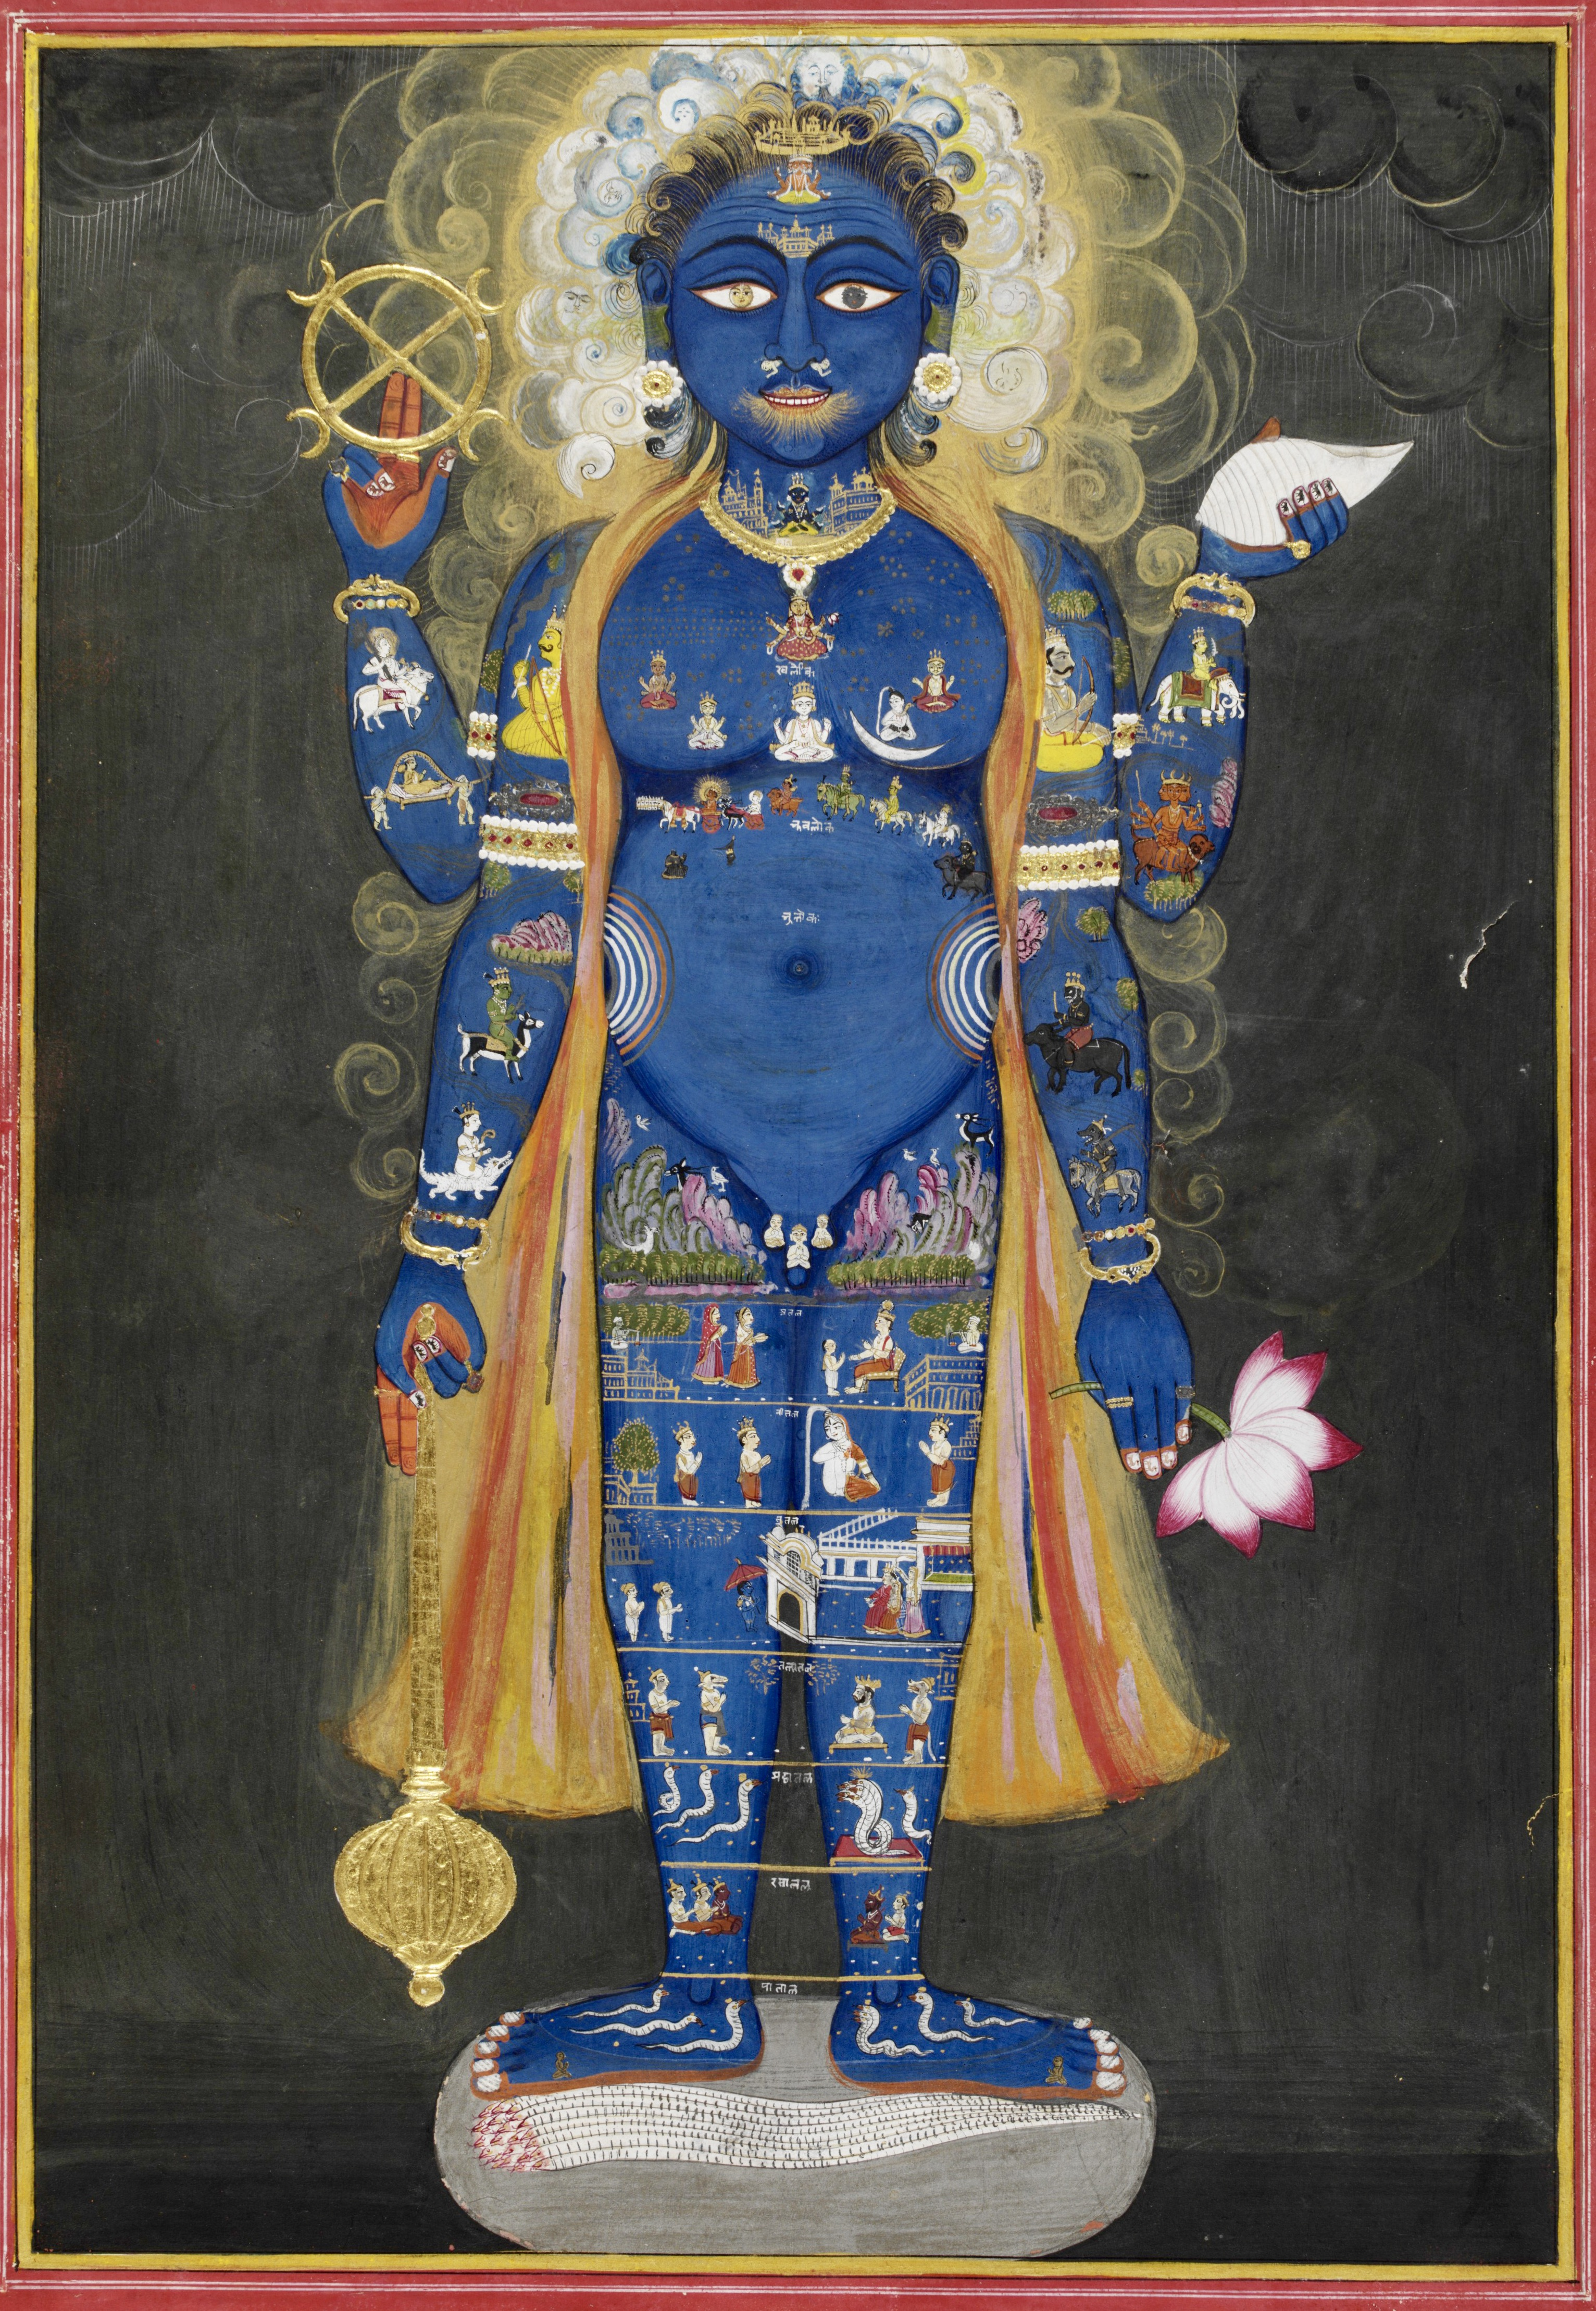
\includegraphics[width=1\textwidth]{pics/Vishnu_Vishvarupa_cropped.jpg}
	\caption{Viṣṇu Viśvarūpa, India, Rajasthan, Jaipur, ca. 1800–1820, Opaque watercolor and gold on paper, 38.5 × 28 cm, Victoria and Albert Museum, London, Given by Mrs. Gerald Clark.}
	\label{fig1}
      \end{figure}
\clearpage
  \begin{figure}[ht]
	\centering
  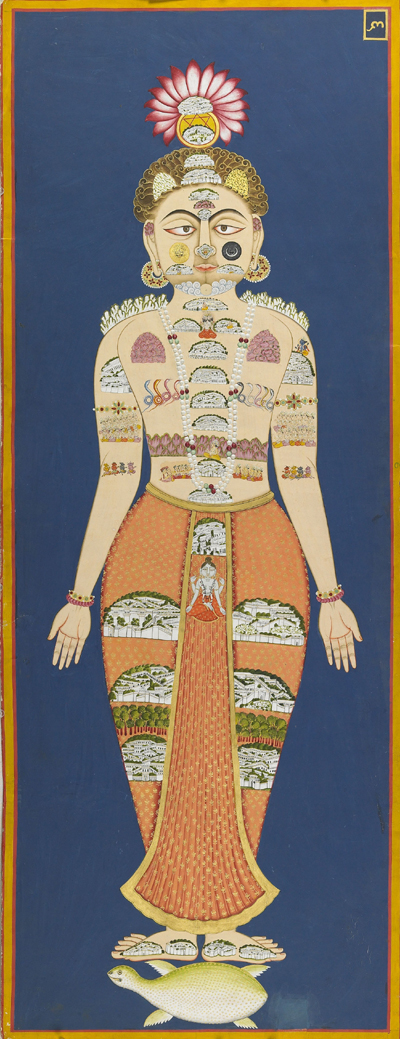
\includegraphics[width=0.5\textwidth]{pics/The_Equivalence_of_Self_and_Universe_(detail),_folio_6_from_the_Siddha_Siddhanta_Paddhati,_(Bulaki),_1824_(Samvat_1881);_122_x_46_cm._Mehrangarh_Museum_Trust..jpg}
	\caption{The Equivalence of Self and Universe (detail), folio 6 from the \textit{Siddhasiddhāntapaddhati} (Bulaki), India, Rajasthan, Jodhpur, 1824 (Samvat 1881), 122 x 46 cm, RJS 2378, Mehragarh Museum Trust.}
	\label{fig2}
      \end{figure}
      % \end{landscape}


\chapter{Bibliography}
 \label{sec:bibli}
   \clearpage
\newpage 
\thispagestyle{empty}
\quad  \addtocounter{page}{-1}

\printbibliography[heading=subbibintoc, title=Consulted Manuscripts, keyword=codex]

\printbibliography[heading=subbibintoc, title=Printed Editions, keyword=printsource]

\printbibliography[heading=subbibintoc, title=Secondary Literature, keyword=seclit]

\printbibliography[heading=subbibintoc, title=Online Sources, keyword=onlinesource]

\end{document}
